\documentclass{book}
\usepackage{graphicx} % Required for inserting images
\usepackage{amsfonts}
\usepackage{amsmath}
\usepackage{amssymb}
\usepackage{listings}
\usepackage{xcolor}


\title{Sistemi elettronici programmabili}
\author{Marco C}
\date{March 2025}



\begin{document}
%Verilog color
\definecolor{backcolour}{rgb}{0.95,0.95,0.92}
\definecolor{vgreen}{RGB}{104,180,104}
    \definecolor{vblue}{RGB}{49,49,255}
    \definecolor{vorange}{RGB}{255,143,102}
    \lstdefinestyle{verilog-style}
    {
        backgroundcolor=\color{backcolour},   
    commentstyle=\color{vgreen},
    keywordstyle=\color{vblue},
    numberstyle=\tiny\color{vorange},
    stringstyle=\color{vorange},
    basicstyle=\ttfamily\footnotesize,
    breakatwhitespace=false,         
    breaklines=true,                 
    captionpos=b,                    
    keepspaces=true,                 
    numbers=left,                    
    numbersep=5pt,                  
    showspaces=false,                
    showstringspaces=false,
    showtabs=false,                  
    tabsize=2
    }
    \lstset{style=verilog-style}

\maketitle

\section*{Disclaimer}
    Questi appunti sono da prendere come riferimento per fare l'esame, ma per una conoscenza approfondita è meglio consultare il libro di Napoli da cui ho preso le informazioni, xoxo.
\chapter{Flusso di progetto per circuiti digitali}

\section{Front-end e back-end di un flusso di progetto}
    Il flusso di progetto per circuiti digitali programmabili ha una faccia del genere:
    \begin{figure}[h!]
        \centering
        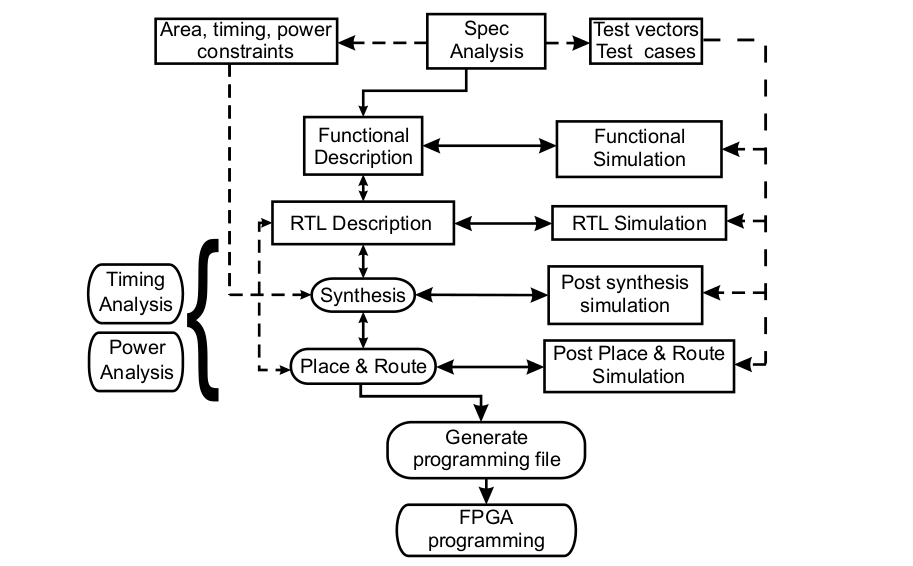
\includegraphics[width=0.75\linewidth]{img/chapt3img1.png}
        \caption{Flusso di progetto di un circuito digitale. Le fasi cerchiate in rettangolare le fa il progettista mentre quelle più rotonde sono semiautoatiche.}
    \end{figure}
    La parte di front-end è orientata alla descrizione del circuito, implementazione degli algoritmi e alla simulazione dello stesso. Essa si conclude con la definizione dei blocchi logici da utilizzare, che dipendono dall'offerta della tecnologia che si sta usando, unico caso in cui c'è dipendenza del front-end dalla tecnologia. Il back-end si occupa invece della progettazione e della verifica relativa alla struttura del circuito, che è la progettazizione delle maschere per ASIC, lo stampo della PCB per i discreti eccetera.
\section{Analisi delle specifiche}
    In questa fase si definiscono le specifiche del circuito da progettare. Per esempio in un device dedito al processing di immagini queste potrebbero essere la risoluzione, la profondità di bit etc...; successivamente si analizzano i costraint dati dal cliente quali possono essere area, tempi di propagazione e potenza dissipata. In particolare l'area dipende anche dalla tecnologia di FPGA scelta per il prototipo, perché si avranno limitazioni circa i blocchi digitali disponibili per organizzare il progetto. La terza cosa da fare è progettare in che modo verificare come si comporta il circuito in determinate situazioni e fare il test per la presenza di errori. Questa cosa viene fatta tramite l'introduzione dei test vector/test case, cioè input di cui si conosce l'output previsto, il quale si confronta con quello effettivo per verificare la presenza di errori.
\section{Descrizione funzionale}
    A questo punto bisogna utilizzare un HDL (Hardware Description Language) per organizzare il progetto in uno schema a blocchi. Si tenga conto che non tutti i costrutti dell'HDL sono direttamente traducibili in circuito digitale. A questo punto si fanno uno o più \textit{test bench} scritti in HDL. Un test bench corrisponde all'inieizione all'interno del circuito di un test vector e confrontare le uscite con i risultati attesi.
    \begin{figure}[h!]
        \centering
        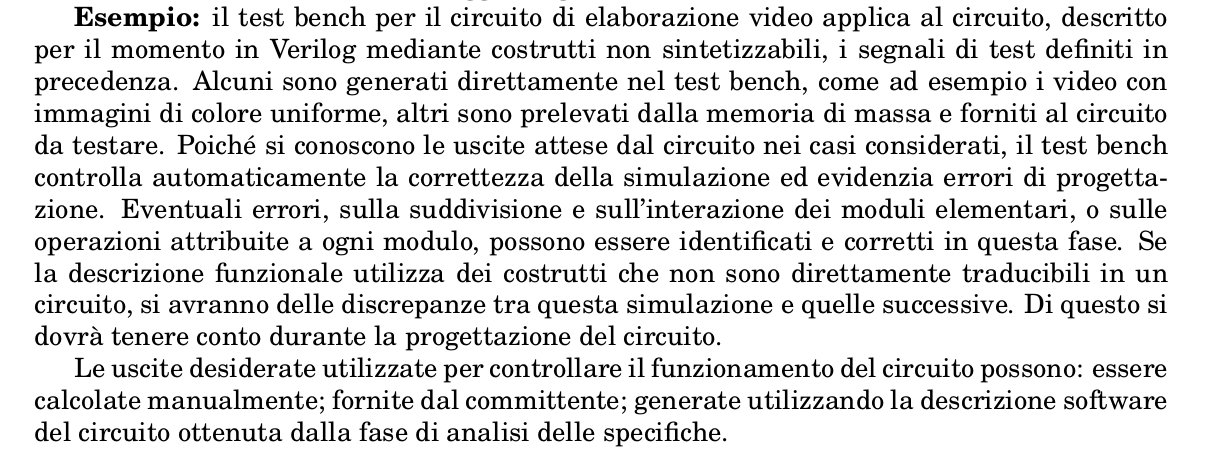
\includegraphics[width=1.1\linewidth]{img/chapt3img2.png}
    \end{figure}
\section{Descrizione RTL}
    In questa fase tutti i blocchi circuitali, anche quelli non sintetizzabili, devono essere espressi come circuito. Allora si sfrutta l'HDL con cui si è già fatto il "design" ideale del progetto per ottimizzare le parti inutili e cercare di tradurre i blocchi logici non direttamente sintetizzabili. In questa parte l'HDL si occupa di tradurre i blocchi logici in costrutti formati da operatori, shift register eccetera. Inoltre, vengono definiti il numero di cicli di clock necesari per compiere determiante operazioni e assieme a quali sezioni del circuito è opportuno ripetere (tecnica di ridondanza). Per vedere se tutto è andato bene, si procede con la simulazione RTL per verificare che la transizione da HDL a circuito digitale è andato a buon fine. Spesso l'analisi funzionale e quella RTL sono fatte con lo stesso software in quanto è di solito compito del programmatore scegliere esplicitamente di effettuare quella funzionale, rendendo de facto simulazione RTL e funzionali sinonimi. La RTL è più veloce e non da informazioni sui parametri del circuito quali potenza o area occupata, ma fornisce dati circa il throughput, la latenza e la sincronizzazione tra i blocchi.
    \begin{figure}[h!]
        \centering
        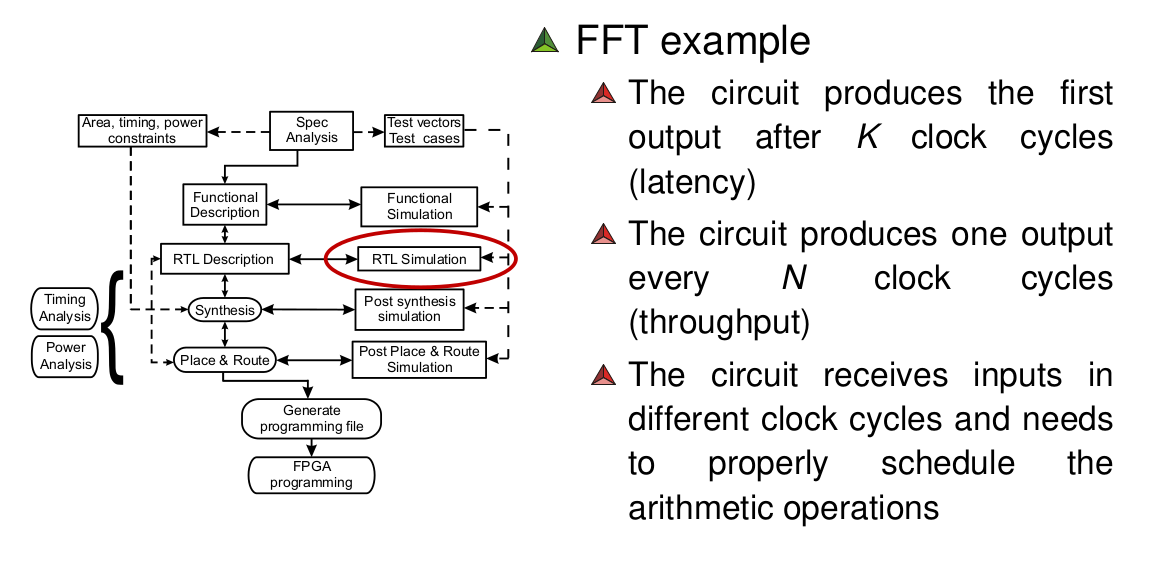
\includegraphics[width=0.95\linewidth]{img/chapt3img3.png}
    \end{figure}
\section{Sintesi}
    Nella fase di sintesi i blocchi funzionali del circuito digitale sono tradotti in componenti digitali. È divisa in due fasi. La prima, detta di \textit{translate}, traduce i blocchi logici in componenti digitali totalmente generici che possono essere implementati da qualunque device FPGA che utilizza liberie standard per circuiti VLSI. La seconda fase, detta di \textit{mapping}, associa ai componenti generici i componenti che sono effettivamente disponibili all'interno del dispositivo FPGA in esame. A volte c'è corrispondenza diretta, come un flip-flop per rappresentare un elemento ad un bit di memoria, mentre altre volte bisogna tradurre un blocco non sintetizzabile in altri modi, per esempio utilizzando una memoria per tradurre una logica combinatoria complessa. Alla fine della fiera si ottiene una \textit{netlist}, ovvero una lista di connessioni sottoforma di file ASCII, che è un elenco degli ingressi, uscite e dei fili che collegano i vari componenti.
\section{Simulazione post-sintesi}
    La simulazione post-sintesi viene fatta per:
    \begin{itemize}
        \item Individuare eventuali bug nella netlist, cioè errori nella fase di translate o di mapping
        \item Avere informazioni sul consumo di potenza, tenendo conto dei glitch (commutazioni multiple dello stesso segnale) e dei tempi di propagazione, che in questa fase possono misurati
        \item Se si è utilizzato il clock gating\footnote{In computer architecture, clock gating is a popular power management technique used in many synchronous circuits for reducing dynamic power dissipation, by removing the clock signal when the circuit, or a subpart of it, is not in use or ignores clock signal.}, questo si può simulare.
\section{Place and route}
    Durante il place and route vengono piazzti (place) i componenti del circuito nelle zone a cui appartengono ed effettuati i collegamenti (route) fra di essi. Questa fase è dispendiosa in termini di potenza di calcolo perché, non esistendo algoritmi in grado di minimizzare l'area occupata e la lunghezza dei cavi conoscendo soltanto i pezzi da utilizzare, quello che si fa è try and error finché non si riduce man mano l'area. Questa cosa richiede uno sforzo di calcolo assurdo ed al progettista è chiesto soltanto, in questa fase praticamente automatica, di indicare quanto tempo e potenza di calcolo dare al programma per trovare il setup migliore, cioè quando questo deve sforzarsi. Tipicamente il massimo sforzo per il Place and Route si fa alla fine, quando si è sicuri di non dover modificare più niente. Come sempre si fa alla fine una simulazione post-P\&R che segnala eventuali errori nelle connessioni. In questa simulazione qua l'accuratezza con cui si può calcolare potenza e tempi di propagazione è massima, perché gli effetti parassiti dei componenti si conoscono. Il check sul tempo di propagazione massimo, che si ha per il percorso critico, si fa durante la \textit{time-analysis}, mentre quello per la potenza dissipata durante il \textit{power-analysis}. Se il circuito non passa una di queste due, bisogna tornare indietro alla fase di progetto RTL e rivalutare le proprie scelte.
\section{Generazione del file FPGA e programmazione}
    Se tutto è andato bene con la post-P\&R analysis, si può generare il bitstream e caricarlo all'interno della FPGA, che viene programmato automagicamente.
    \end{itemize}

\chapter{Field Programmable Gate Array}
    Gli FPGA sono dispositivi elettronici programmabili, chiamati così perché derivanti dai Gate Array e programmabili direttamente sul proprio tavolo da lavoro. L'utlizzo della parola "programmare" riferita ad un FPGA è fuorviante, in quanto un progettista FPGA si occupa di organizzare i collegamenti del circuito e la scelta dei componenti, ottenendo come risultato un circuito digitale, a differenza di qualcuno che programma in linguaggi come il C o l'assembly, per i quali "programmare" significa elencare una serie di istruzioni da fare eseguire ad un computer.
\section{Struttura di un FPGA}
    Ci sono tre layout principali per la struttura di un FPGA:
    \begin{figure}[h!]
        \centering
        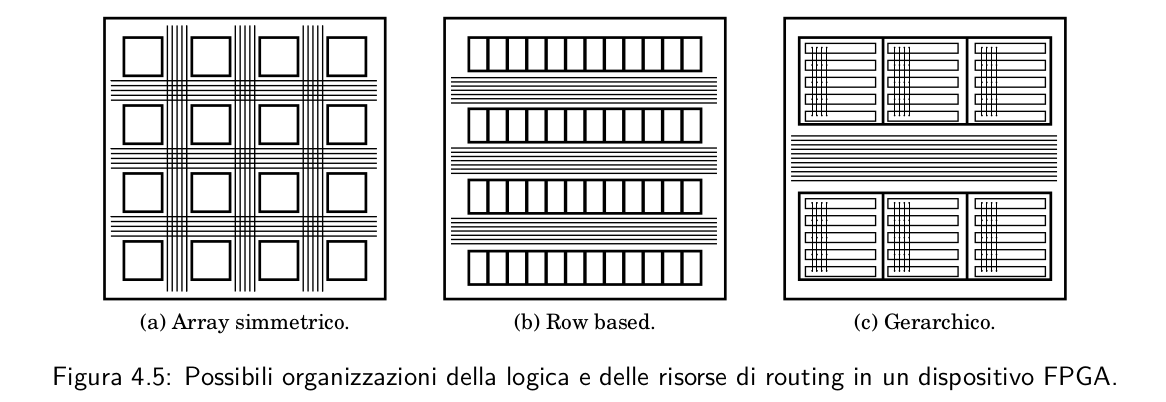
\includegraphics[width=0.75\linewidth]{img/chapt4img1.png}
    \end{figure}
    La disposizione a matrice e quella a righe sono alquanti simili e differiscono solo per il fatto che nella prima i percorsi logici si intrecciano ad ogni intersezione, mentre per la seconda sono compresi fra due righe di elementi logici. La terza, quella gerarchica, è fondamentalmente diversa. La struttura è a righe, ma ogni blocco logico ha una sottostruttura a righe di media complessità logica costituita da blocchi logici a loro volta costituiti da una sottostruttura e così via.\\
    Le FPGA si possono distinguere anche a seconda del fatto che siano programmabili una sola o più volte, oppure che siano volatili e non:
    \begin{figure}[h!]
        \centering
        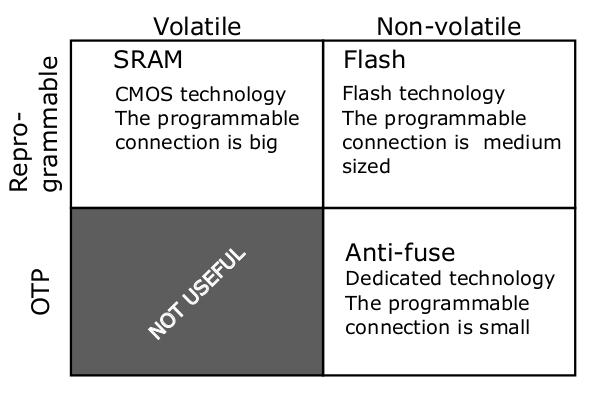
\includegraphics[width=0.75\linewidth]{img/chapt4img2.png}
        \caption{I vari modi per distinguere un FPGA}
    \end{figure}\\
    Un esempio di FPGA programmabile più volte e volatile è quello basato su SRAM. Il bitstream viene caricato e ogni celletta di SRAM conserva un dato che identifica se una connessione deve essere aperta o chiusa tramite porta di trasmissione CMOS.
    \begin{figure}[h!]
        \centering
        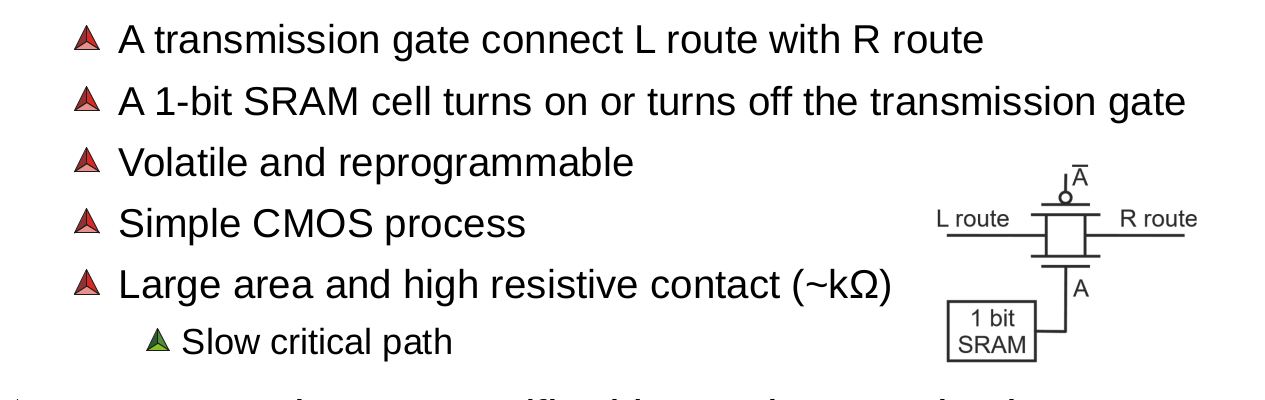
\includegraphics[width=0.75\linewidth]{img/chapt4img3.png}
    \end{figure}\\
    È necessaria una memoria flash esterna per conservare la configurazione, che viene caricata in memoria dinamica ogni volta.\\
    Un esempio invece di non-volatile OTP è la tecnologia FPGA basata su antifuse. In questo caso si crea un piccolo vuoto nel canale di via tra due layer di metal e dove si vuole fare il collegamento si applica una ddp abbastanza forte che scioglie la via e collega i due layer di metal.
    \newpage
    \begin{figure}[h!]
        \centering
        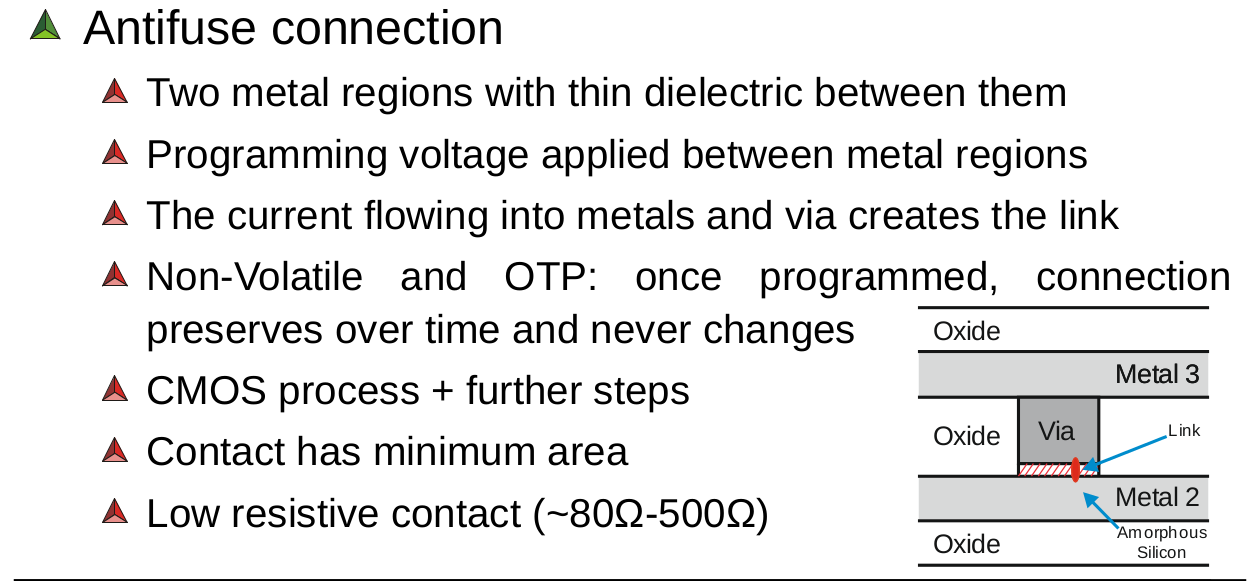
\includegraphics[width=0.75\linewidth]{img/chapt4img4.png}
    \end{figure}
    Un esempio invece di FPGA non-volatile e riprogrammabile è dato da quelli basati su flash switch:
    \begin{figure}[h!]
        \centering
        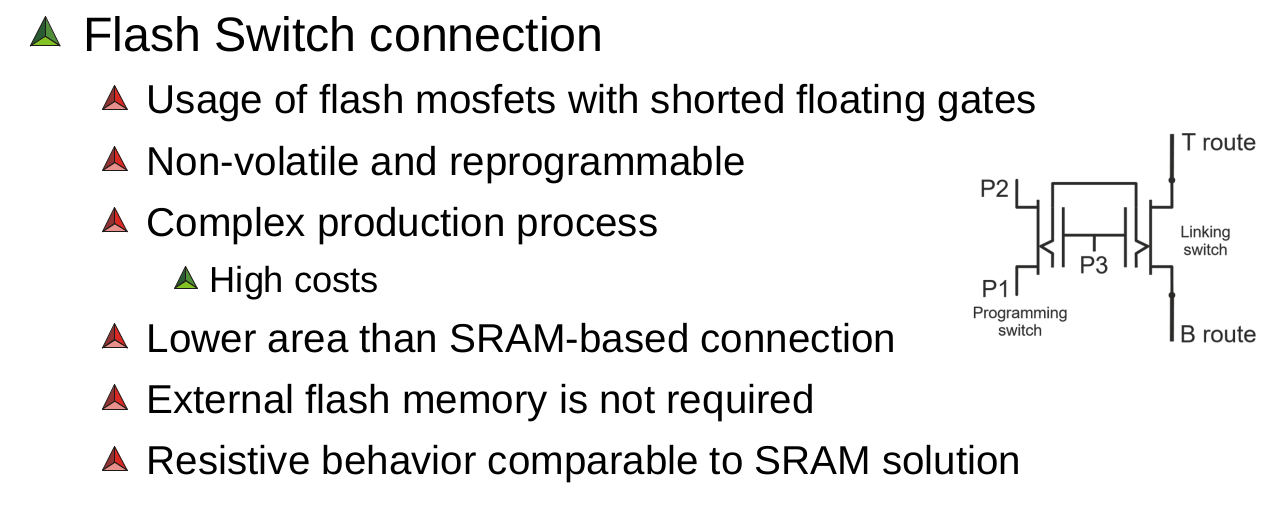
\includegraphics[width=0.75\linewidth]{img/chapt4img5.png}
    \end{figure}
\section{Architettura di celle logiche programmabili}
    Al fine di garantire la massima flessibilità, gli elementi logici che costituiscono un FPGA sono anch'essi programmabili. Ci sono due tipi di architetture per le celle logiche: quelle basate su multiplexer e quelle basate su Look Up Tables (LUT). \\
    Le FPGA che utilizziamo noi sono basate su Look-up table. Una LUT è un blocco logico ad $n$ ingressi ed una uscita. La LUT ha un elemento di memoria per conservare $2^{n}$ bit che sono i possibili che può assumere una funzione booleana ad $n$ ingressi, potendo implementare potenzialmente $2^{2^{n}}$ funzioni diverse.
    \\ \\
    Un moderno FPGA si compone dei seguenti elementi:
    \begin{itemize}
        \item I \textbf{Logic Element} (LE), implementati come abbiamo detto in MUX o LUT. Possono essere piccoli blocchi RAM, ROM, shift register...
        \item I \textbf{blocchi RAM} (BRAM), slice di unità o decine di kilobyte di RAM
        \item I \textbf{blocchi DSP}, cioè quelli per il digital signal processing come accumulatori, addizionatori, moltiplicatori...
        \item CPU, che può essere \textit{soft}, cioè implementata tramite i blocchi logici del dispositivo, oppure \textit{hard}, fatta ad-hoc per il device. Le prime sono più lente ma possono essere customizzate a seconda delle necessità.
    \end{itemize}
    Sulla parte periferica del chip FPGA troviamo:
    \begin{itemize}
        \item I \textbf{banchi I/O} che sono altamente programmabili per tutte le stronzate che ti passano in mente: gestione della reiezione del rumore, direzione dell'IO, valori di corrente eccetera.
        \item Il \textbf{clock management}, che si occupa di trasferire il segnale di clock all'FPGA. Il CM può ritardare, moltiplicare e fare altre operazioni sul segnale di clock.
        \item \textbf{High speed IO} per il trasferimento seriale ad alta velocità.
    \end{itemize}
\section{Caratteristiche delle celle logiche programmabili}
    Gli elementi sequenziali sono d'importanza fondamentale. Sebbene si possa pensare in un primo momento di poter implementare un flip flop tramite inverttitori classici e collegamenti programmabile, ciò riduce il numero di celle logiche disponibili e da molta difficoltà nella gestione del timing. Allora i programmatori di FPGA preferiscono implementare i Flip-Flop nativamente nei loro logic element (LE). Questi flip-flop infatti devono essere pianamente programmabili e si deve poter decidere su quali fronti di clock farli lavorare, se usare un segnale S/R eccetera.\\ \\
    Generalmente gli LE implementano funzioni combiantorie. In alcune schede gli LE sono chiamati Slice. Dunque ogni Slice/LE ha delle LUT e dei flip-flop:
    \begin{figure}[h!]
        \centering
        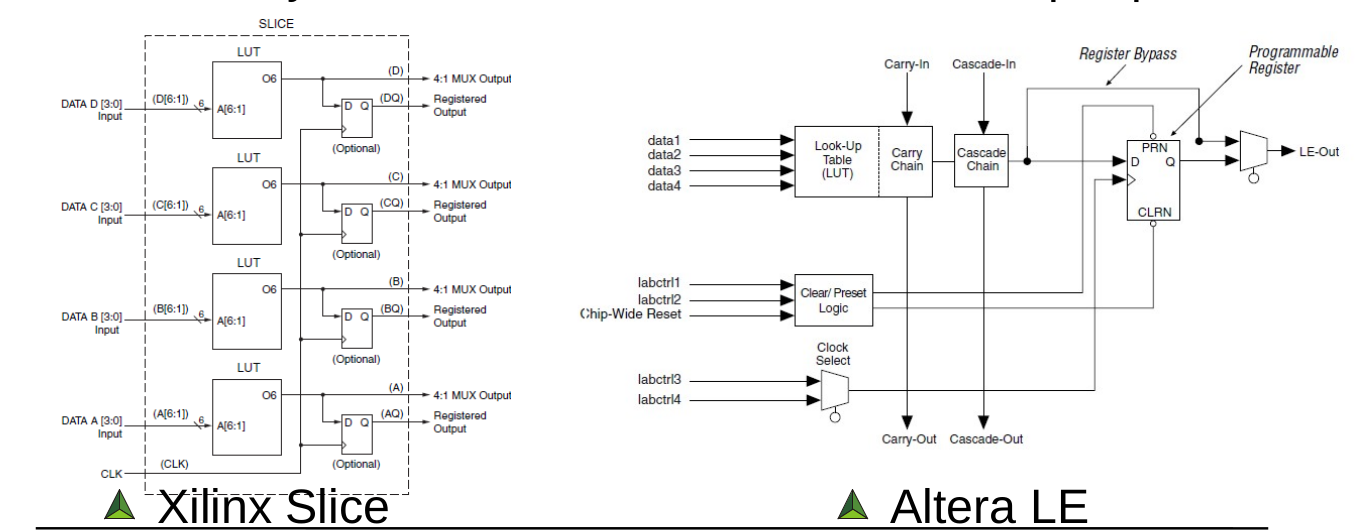
\includegraphics[width=0.95\linewidth]{img/chapt4img6.png}
    \end{figure}
    \begin{figure}[h!]
        \centering
        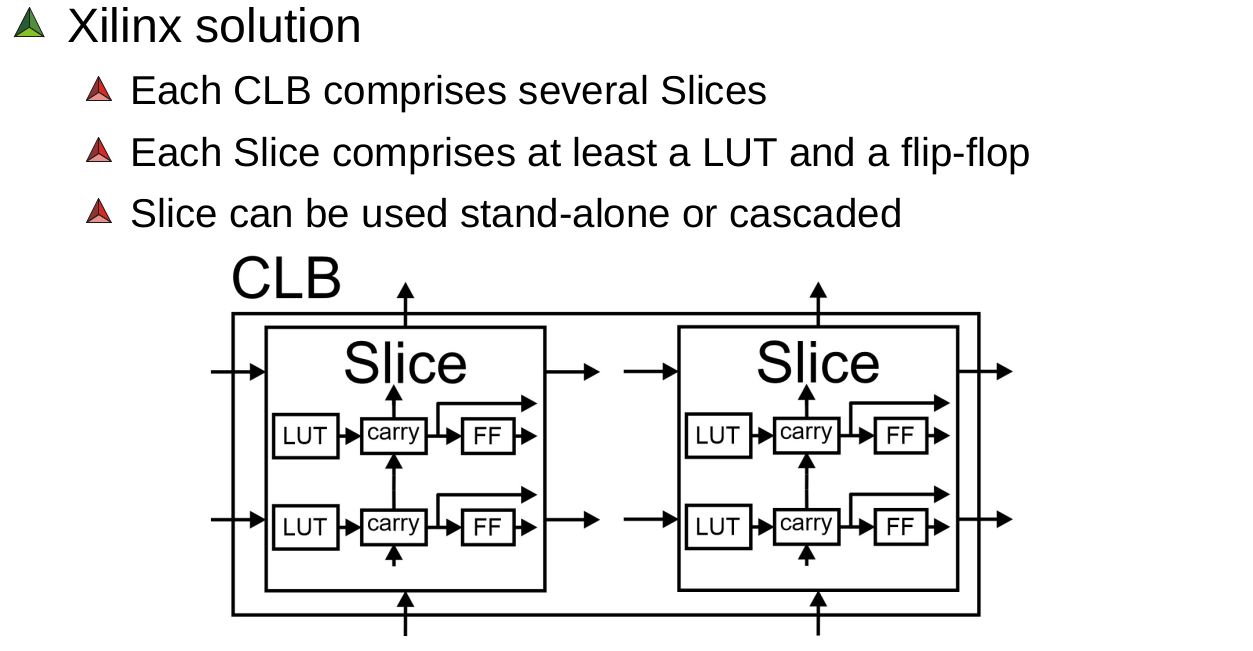
\includegraphics[width=1\linewidth]{img/chapt4img8.png}
    \end{figure}
    \begin{figure}[h!]
        \centering
        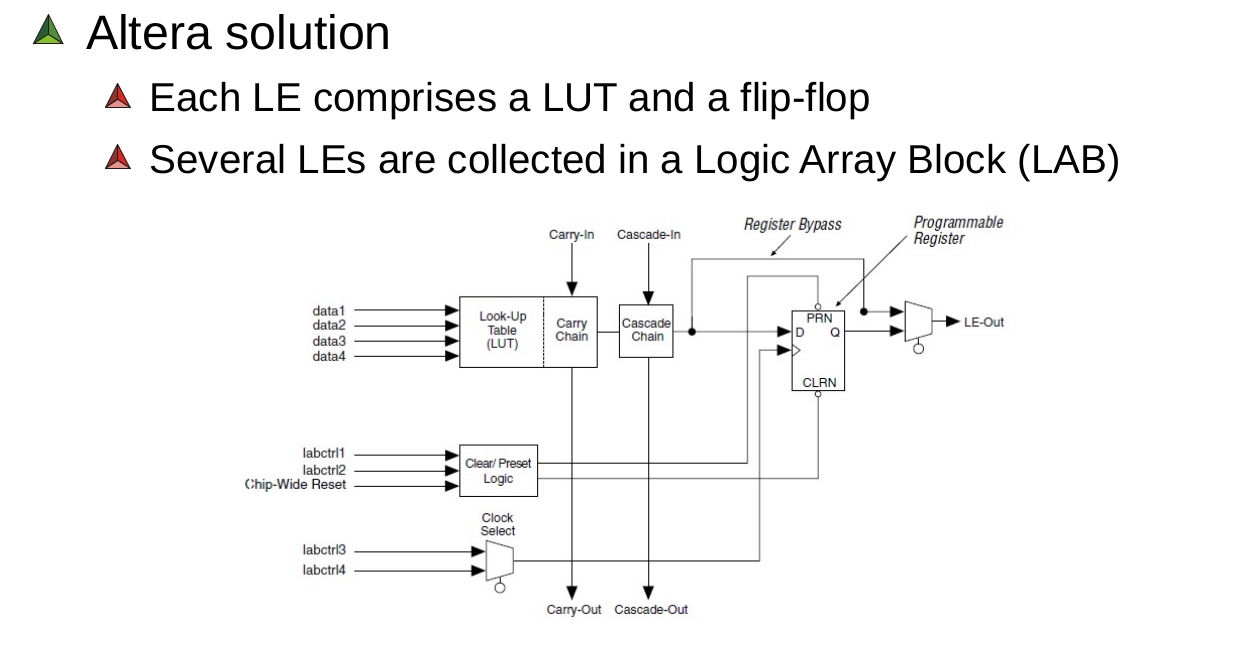
\includegraphics[width=1\linewidth]{img/chapt4img9.png}
    \end{figure}
    \newpage
    Le FPGA ad alte prestazioni implementano gli ALM (Adaptive Logic Module):
    \begin{figure}[h!]
        \centering
        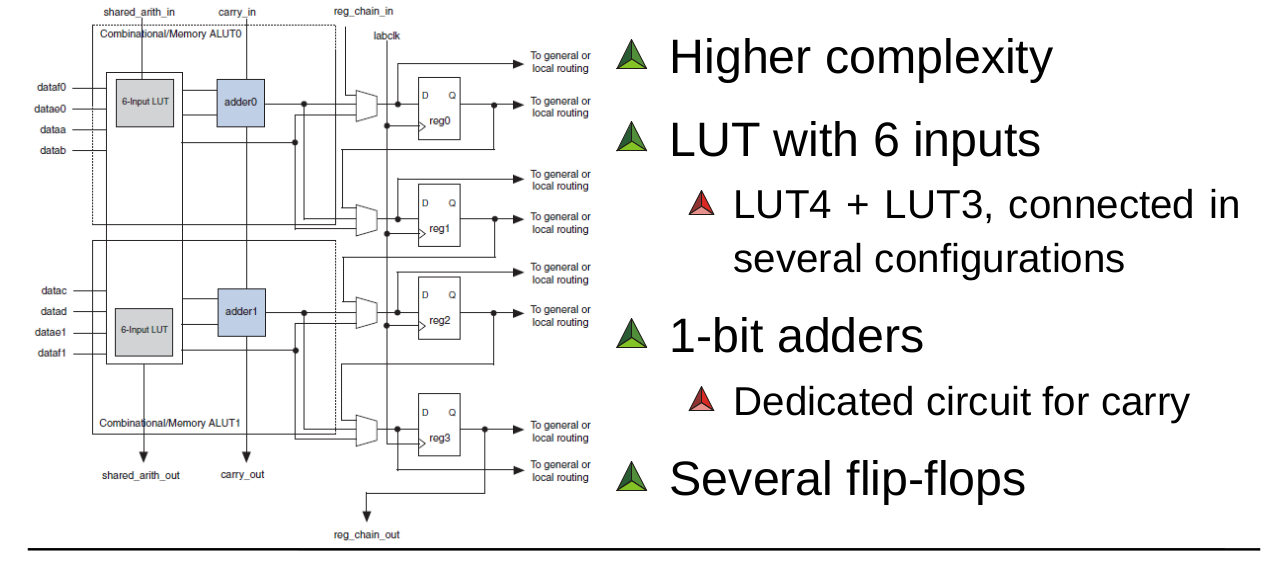
\includegraphics[width=0.75\linewidth]{img/chapt4img10.png}
    \end{figure} \\
    Questo tipo di elemnti logici hanno al loro interno LUT adattabili, nel caso di Altera si può scegliere di utilizzare LUT4, LUT5 o LUT6 collegando in cascata delle LUT4. \\ \\
    Gli addizionatori nei circuiti digitali sono comuni e si può implementare un adder da un bit utilizzando una LUT4 divisa in due LUT3, una per il risultato della somma di due bit e l'altra per il riporto. Mettendone in cascata $n$, si ottiene un addizionatore ad $n$ bit.
    \begin{figure}[h!]
        \centering
        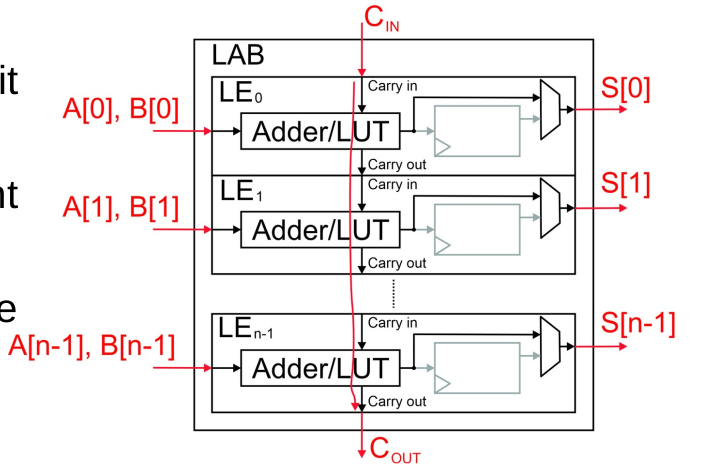
\includegraphics[width=0.75\linewidth]{img/chapt4img11.png}
    \end{figure}
    Negli ALM ci sono circuiti addizionatori dedicati, per garantire migliore flessibilità. Ci sono anche circuiti per la propagazione del riporto (carry-propagation), dunque connettendo $n$ ALM in cascata è possibile creare addizionatori di $2n$ bit. \\ \\
    Le look up table si comportano come piccole memorie RAM e possono essere programmate tramite i registri ProgDIN, ProgCLK, ProgWR, i quali una volta programmata la cella vengono disabilitati, facendo sì che la LUT si comporti come un circuito combinatorio ordinario. Si possono usare allora le LUT come memorie RAM distribuite, i cui bit possono essere scritti a runtime tramite i registri citati sopra.
    \begin{itemize}
        \item \textbf{ProgDin}: registro dato da memorizzare nella RAM.
        \item \textbf{ProgCLK}: registro per temporizzare operazioni di lettura e scrittura.
        \item \textbf{ProgRW}: registro per segnalare stato di lettura o scrittura.
    \end{itemize}
    \newpage
    Le LUT possono essere utilizzate anche per fare RAM dual port e performare lettura e scrittura in contemporanea:
    \begin{figure}[h!]
        \centering
        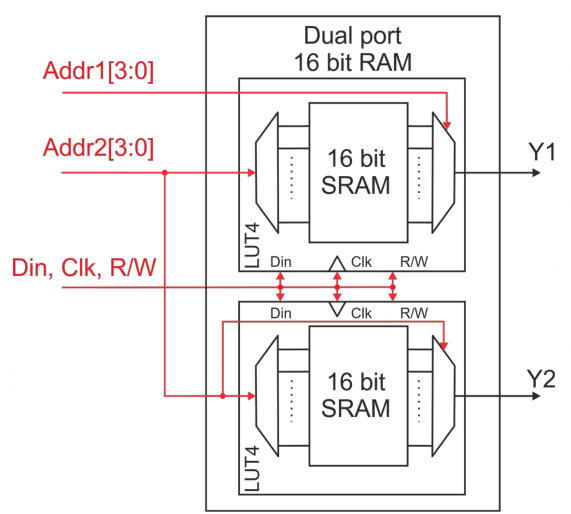
\includegraphics[width=0.75\linewidth]{img/chapt4img12.png}
    \end{figure}
    \\ \\ 
    Per la costruzione di registri a scorrimento, tipicamente si mettono in serie dei flip-flop. Altera ottimizza questa cosa con una circuiteria ad-hoc per le cascade di ALM, mentre altre schede permettono di creare shift-register programmando le varie RAM basate su LUT per tale scopo. In generale con una LUT da $n$ bit si può implementare un registro a scorrimento di $2^{n}$ locazioni di memoria.
\chapter{Circuiti combinatori}
    \section{Multiplexer}
        Un multiplexer (abbreviato in MUX) è un circuito combinatorio. Un circuito combinatorio è un circuito la cui uscita dipende esclusivamente dagli ingressi e non dallo stato corrente del circuito, come invece accade nei circuiti sequenziali. Per questa loro proprietà, i circuiti combinatori non implementano alcun tipo di retroazione. \\ \\
        Un MUX, nella sua forma più generale possibile, è un circuito che ha in ingresso $n$ stringhe da $p$ bit. Il mux instrada uno tra gli $n$ ingressi tramite $p$ bit di selezione e viene detto \textit{completo} se $2^{m} = n$. Per implementare un mux di stringhe a $p$ bit basta mettere in parallelo $p$ mux $n:1$, ognuno controllato dagli stessi $m$ bit e con le uscite preelvate in parallelo:
        \begin{figure}[h!]
            \centering
            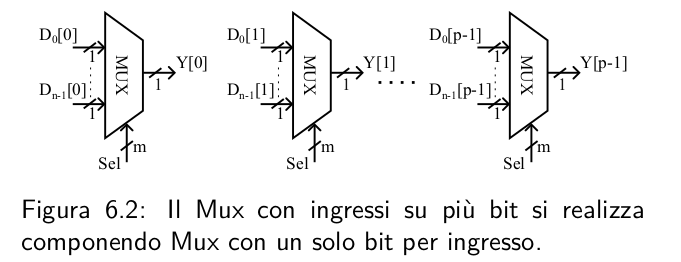
\includegraphics[width=0.75\linewidth]{img/chap6img1.png}
        \end{figure} \\ \\
        Il MUX  $2:1$, il più utilizzato nei circuiti digitali, equivale al costrutto "if-else". Un esempio lo abbiamo con il calcolo del valore assoluto. Se $A$ è il valore del numero ed $S$ il segno di $A$, il MUX $2:1$ implementa una funzione del genere (avendo dato gli ingressi opportuni):
        \begin{equation}
            Y = A\bar{S}+\bar{A}S
        \end{equation}
        cosicché se $A$ è positivo (ed il bit di segno è zero, cioè "+") allora ritorna $A$, altrimenti ritorna il valore di $-A = \bar{A}$, che è positivo se $A$ è negativo, così come il bit di segno $S$ che sarà uguale ad $1$.
    \section{Decoder binario}
        Il decoder binario è un altro circuito altrettanto utilizzato e permette di convertire l'espressione di numeri da un formato a quello binario:
        \begin{figure}[h!]
            \centering
            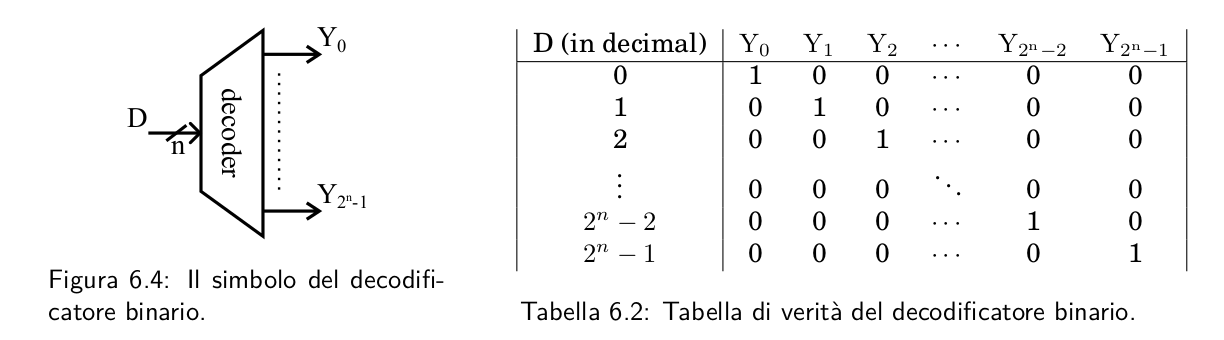
\includegraphics[width=0.75\linewidth]{img/chap6img2.png}
        \end{figure}
        Un utilizzo pratico di un decoder binario lo si trova nelle memorie, dove vengono utilizzati per selezionare le colonne e le righe della matrice di locazioni, che corrisponde all'attivazione dei MOS di riga e di colonna.
    \section{Encoder}
        Un codificatore (encoder) è un qualsiasi circuito che ha in ingresso un codice e lo traduce in un altra rappresentazione. La lunghezza della stringa d'uscita è tipicamente minore di quella d'ingresso, ragion per la quale un encoder non può associare ad ogni ingresso un valore unico di uscita. Per tale ragione, si deve agire in uno dei seguenti modi: o si garantisce che in ingresso al circuito non ci siano ingressi non ammessi oppure si fa in modo che tali ingressi, quando presenti, siano scartati, aggiungendo dei bit all'uscita che ne certifichino l'ammissibilità.\\
        Un esempio di encoder è quello \textit{one-hot}, che ritorna (in binario) la posizione dell'unico uno all'interno della stringa:
        \begin{figure}[h!]
            \centering
            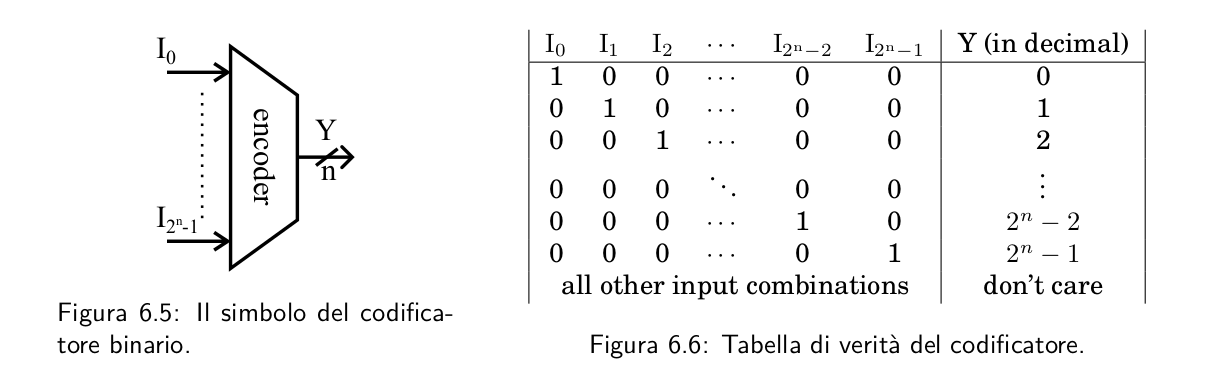
\includegraphics[width=0.75\linewidth]{img/chap6img3.png}
        \end{figure} \\ \\
        L'encoder può essere anche a priorità e viene chiamato in quel caso \textit{priority encoder}. Un priority encoder risolve il problema degli ingressi non validi con più di un bit alto cambiando l'uscita associata alla configurazione con un solo bit alto che ha la priorità maggiore. Se per esempio entra $110$ ed $100$ ha la priorità su $010$, allora l'uscita sarà quella di $100$. Questo meccanismo trova utilizzo nella gestione delle interrupt dei processori, dove il concetto di priorità è di fondamentale importanza. L'enoder a priorità ha lo stesso simbolo dell'encoder normale, eccetto per il segnale di "Idle" disegnato sopra. Il segnale di "Idle" serve a notificare quand'è che l'encoder ha tutti zero in ingresso.
    \section{Comparatore}
        Un comparatore è un circuito che fa un confronto fra due numeri. I comparatori che implementano confronti come l'uguaglianza fra due numeri sono semplici da realizzare, mentre la complessità cresce più che linearmente con l'aumentare dei bit se si prendono comparatori che verificano che un numero sia maggiore di un altro. I comparatori sono di fondamentale importanza nell'implementazione dei cicli, del confronto fra chiavi di sicurezza nella crittografia eccetera. \\ \\
        Un esempio è il comparatore che verifica che un numero sia maggiore di zero. La funzione booleana che implementa questa cosa è:
        \begin{equation}
            IsZero = \bar{I_{0}}\bar{I_{1}} \cdots \bar{I_{n-1}} = \overline{I_{0}+I_{1}+ \cdots + I_{n-1}}
        \end{equation}
        In VLSI la forma NOR è preferita (cioè come prodotto di negati) perché utilizza $2n$ transistor per una funzione ad $n$ ingressi, contro i $4n+2$ utilizzati dalla logica NAND. \\ \\
        Se invece si vuole effettuare il confronto con una costante $C$ diversa da zero, bisogna tener conto di caso per caso. Se la costante, una stringa di $n$ bit, ha meno di $(n+1)/2$ alti, conviene ancora utilizzare la logica NOR, altrimenti è conveniente operare in NAND negando le uscite necessarie. Supponiamo per esempio che $C=110$, allora la funzione da implementare è:
        \begin{equation}
            Y = I_{2}\cdot I_{1} \cdot \bar{I_{0}} = \overline{\bar{I}_{2}+\bar{I_{2}} +I_{0}}
        \end{equation}
        In questo caso conviene una NAND per esempio, mentre se fosse stato, ad esempio, $C=10001$ sarebbe convenuta una NOR. \\ \\
        Per verificare che due segnali $A$ e $B$ siano uguali, bisogna fare il prodotto delle XNOR fra i bit di $A$ e $B$:
        \begin{equation}
            Y = \Pi _{i} ^{n} (A_{i-1} \odot B_{i-1})
        \end{equation}
        dove ricordiamo la XNOR è il negato della NOR, dunque è alta se i due bit sono uguali.\\
        Per relazioni maggiore/minore, ad esempio $A>B$, il circuito è più complesso e richiede oltre s XNOR e AND svariate porte OR.
    \section{Full adder}
        Un full-adder, cioè un addizionatore completo, è un circuito che ha in ingresso tre bit, $A$, $B$, $C_{in}$, con $C_{in}$ il riporto in ingresso, e da in uscita su due bit la somma $S$ e il riporto di uscita $C_{out}$. Ovviamente il bit somma ha più peso del carry di uscita e dunque il full-adder viene spesso chiamato compressore $3:2$, perché comprime un informazione su $3$ bit di peso unitario in una su due bit di peso diverso.
        \begin{figure}[h!]
            \centering
            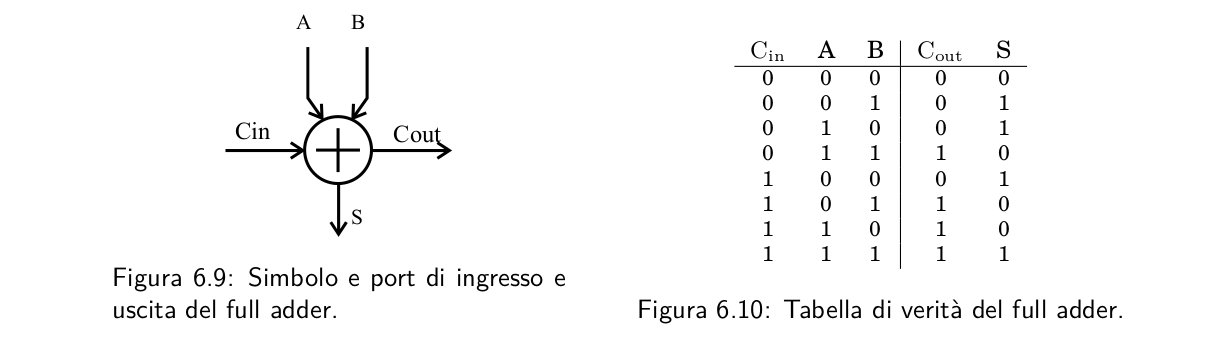
\includegraphics[width=0.75\linewidth]{img/chap6img4.png}
        \end{figure}
\chapter{Introduzione al Verilog}
    \section{Caratteristiche di un HDL}
        Il Verilog è un HDL e dunque permette la descrizione di circuiti digitali e di comportamento, a seconda del livello di astrazione con cui si lavora. Utilizzare un HDL conviene proprio perché si possono descrivere funzioni booleane nel modo più low level possibile, così come sono molto utili i costrutti per la descrizione comportamentale (behavioral constructs). Assieme al VHDL, il Verilog è uno standard industriale per la progettazione di FPGA, CPLD ed ASIC. \\ \\
        Cosa rende un HDL diverso (e più adatto per il low level) da un linguaggio di programmazione software è la possibilità di eseguire istruzioni in parallelo, cosa fondamentale nei circuiti e non presente nei linguaggi software che sono rigorosamente sequenziali. Gli HDL possono essere utilizzati per simulare il comportamento del circuito includendo anche i ritardi, tramite costrutti di simulazione, inoltre sono capaci di effettuare la sintesi circuitali tramite appositi costrutti di sintesi. \\ \\
        L'HDL può essere utilizzato anche per il calcolo di vettori di test, ma quando si passa alla descrizione RTL bisogna ripulire il codice Verilog da costrutti non sintetizzabili. Nelle fasi di sintesi, P\&R e avanti non viene più scritto codice HDL. \\ \\
    \newpage
    \section{Come si descrive un circuito}
        Tutti i file verilog che descrivono circuiti iniziano con la keyword $module$.
        \begin{figure}[h!]
            \centering
            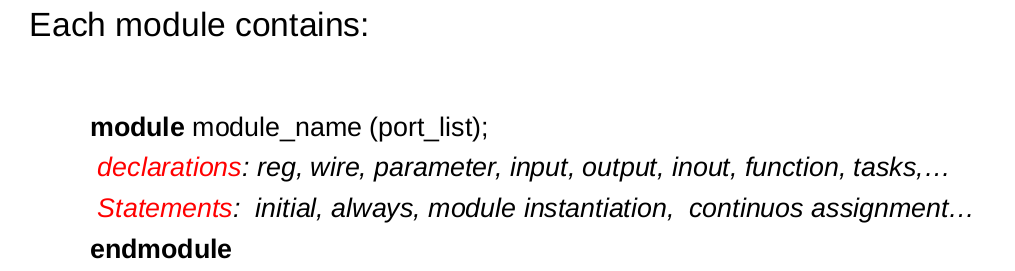
\includegraphics[width=0.75\linewidth]{img/chapt7img1.png}
            \caption{Initial è un esempio di costrutto non sintetizzabile che va rimosso in fase di sintesi}
        \end{figure} \\
    Un esempio facile è il decoder 2:4
    \begin{figure}[h!]
        \centering
        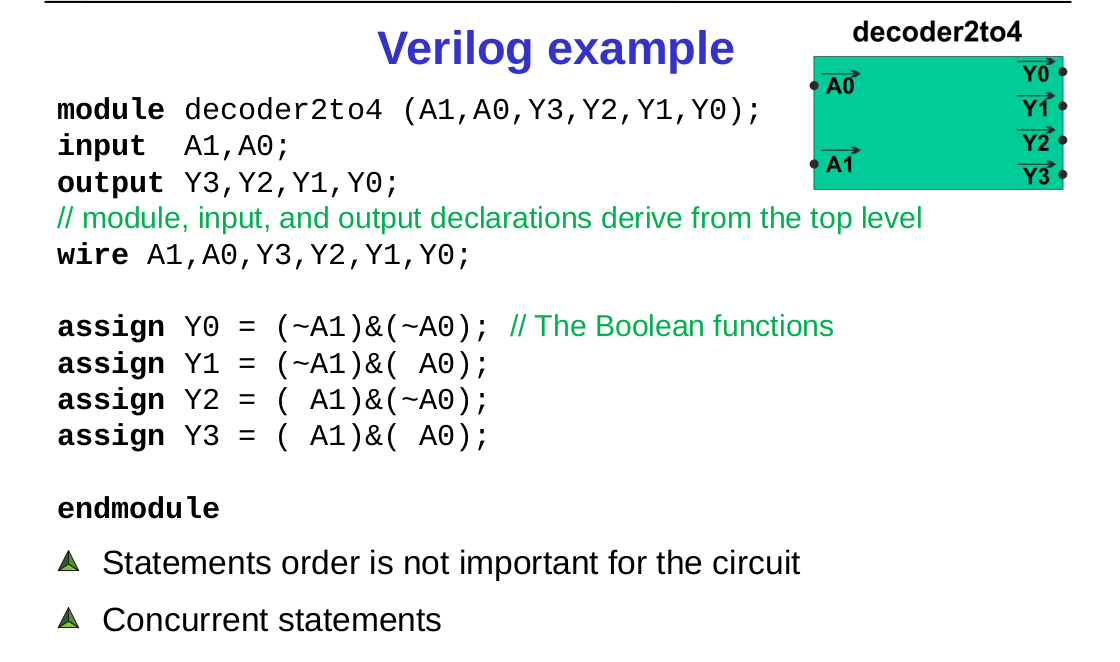
\includegraphics[width=0.75\linewidth]{img/chapt7img2.png}
    \end{figure}
    Prima di scrivere il codice va sempre fatto lo schema a blocchi. Partiamo per esempio dalla tabella di verità e ricaviamo:
    \begin{align}
        y_{0} = \bar{a_{0}}\bar{a_{1}} \\
        y_{1} = a_{0}\bar{a_{1}} \\
        y_{2} = \bar{a_{0}}a_{1} \\
        y_{3} = a_{0}a_{1} \\
    \end{align}
    \\ e quindi la implementiamo all'interno del codice. Allora mi servono 4 LUT per fare le AND da due e 2 LUT per fare gli inverter. \newpage
    Lo stesso circuito si può descrivere con i bus array, definendo quindi due vettori $A$ ed $Y$ che sono i bus rispettivamente di entrata ed uscita:
    \begin{figure}[h!]
        \centering
        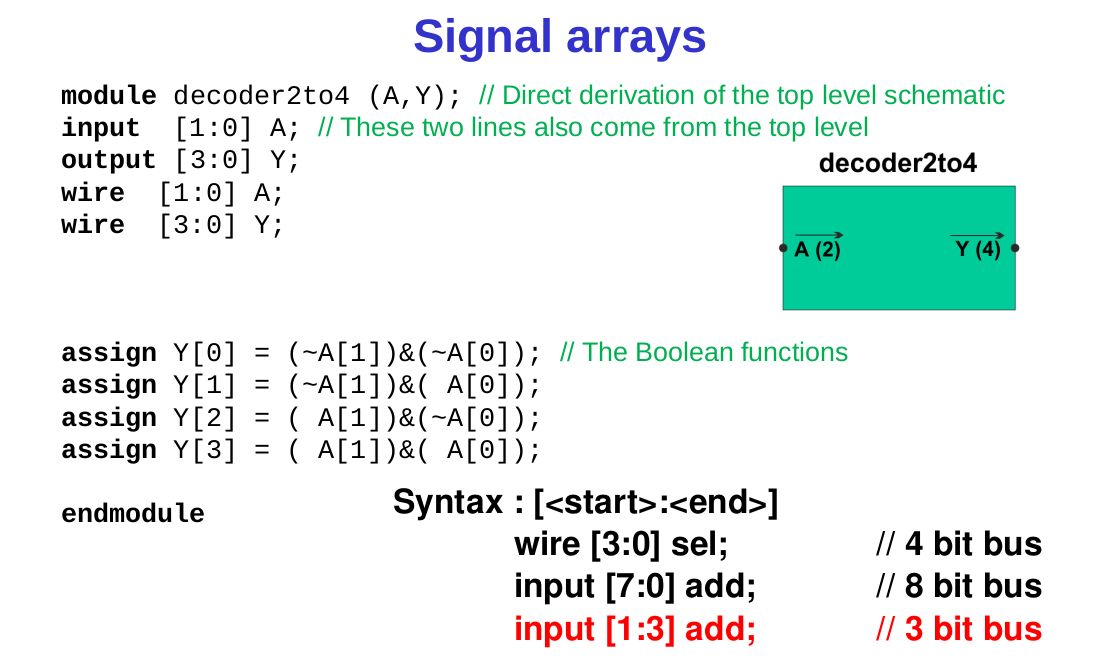
\includegraphics[width=0.75\linewidth]{img/chapt7img3.png}
    \end{figure}

    \section{Descrizione gerarchica}
        La descrizione gerarchica è conveniente perché è complicato lavorare con codici lunghi e anche perché i pezzi che compongono la struttura totale possono essere riutilizzati\footnote{equivalente della modularità per programmi software}. \\
        La keyword che consente di richiamare all'interno di un top level (circuito a gerarchia maggiore) un circuito lower level (un sottocircuito più elementare) é:
        $$
        <module name> <istance name>(<interface \ ports>)
        $$
        Il modulo da mette è quello lower level, poi va istanziato un oggetto che ha le caratteristiche di quel modulo e infine vanno messe le interface ports, che descrivono in che modo si collegano i segnali IO del modulo istanziato. \newpage
    \section{Blocchi procedurali}
        I costrutti verilog sono concorrenti: l'esecuzione dei costrutti è parallela e l'ordine con cui vengono dichiarati i costrutti non variano il funzionamento. Le istruzioni all'interno del blocco procedurale, però, sono sequenziali. Post-sintesi non c'è più il blocco procedurale ma un circuito.\\
        \begin{figure}[h!]
            \centering
            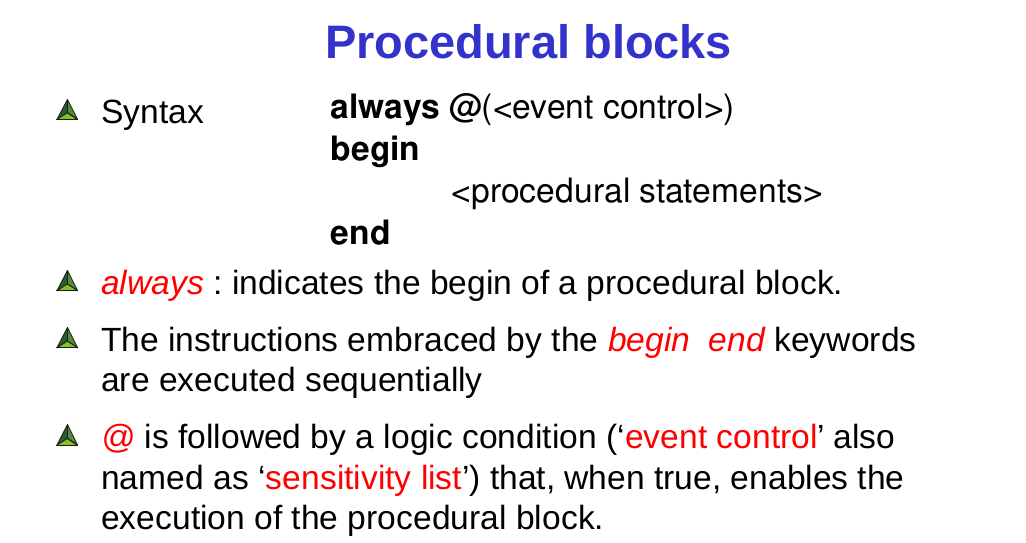
\includegraphics[width=0.60\linewidth]{img/chapt7img4.png}
        \end{figure}
        Un segnale prodotto da un blocco procedurale deve essere definito come \textit{reg}, ma ciò non vuol dire che \textit{reg} sia un registro, semplicemente è un segnale che esce da un blocco procedurale.
        \begin{figure}[h!]
            \centering
            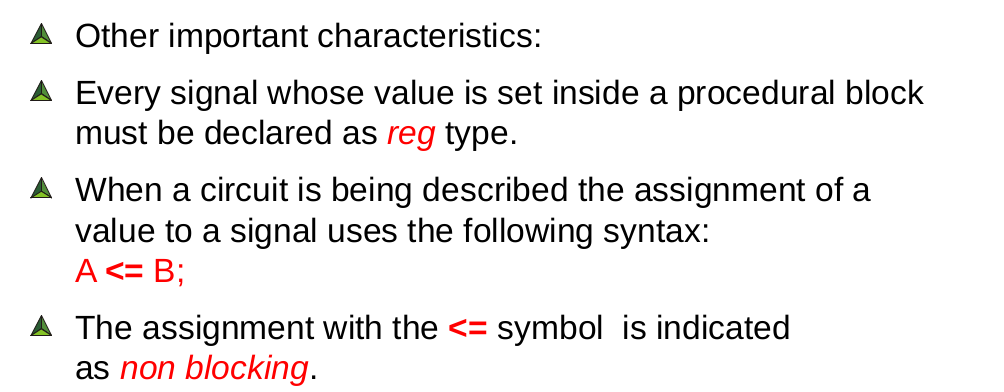
\includegraphics[width=0.5\linewidth]{img/chapt7img5.png}
        \end{figure}
        \begin{figure}[h!]
            \centering
            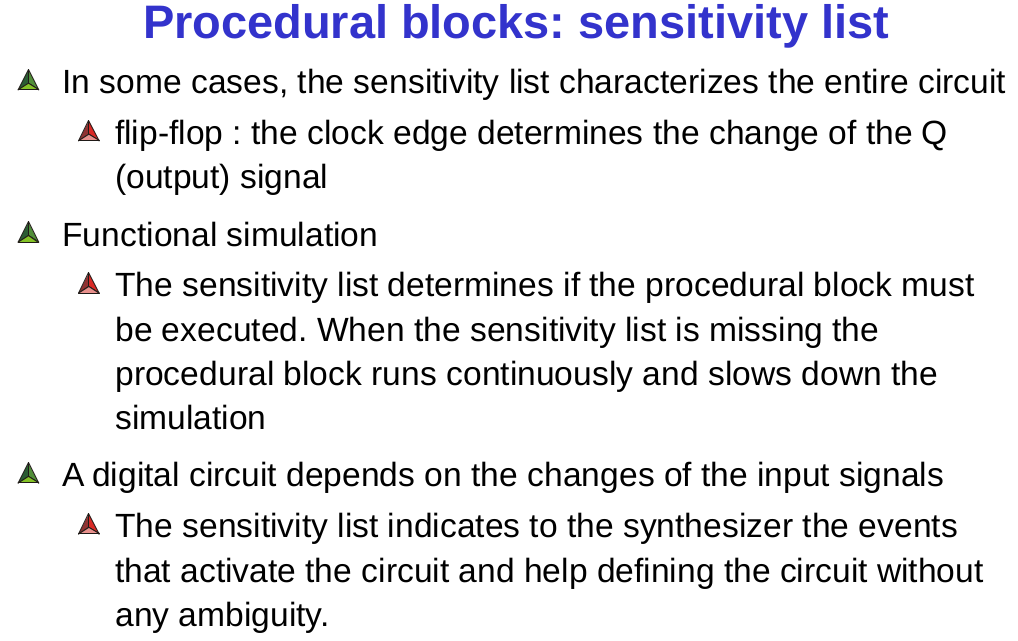
\includegraphics[width=0.5\linewidth]{img/chapt7img6.png}
        \end{figure} \newpage
        Un esempio dove è corretto utilizzare una sensitivity list incompleta è quello del flip flop di tipo D sul fronte di salita. I segnali d'ingresso sono il dato ed il clock, ma l'ingresso può variare soltanto sul fronte di salita del clock (cosa stabilità all'interno del verilog con la keyword $posedge$):
        \begin{figure}[h!]
            \centering
            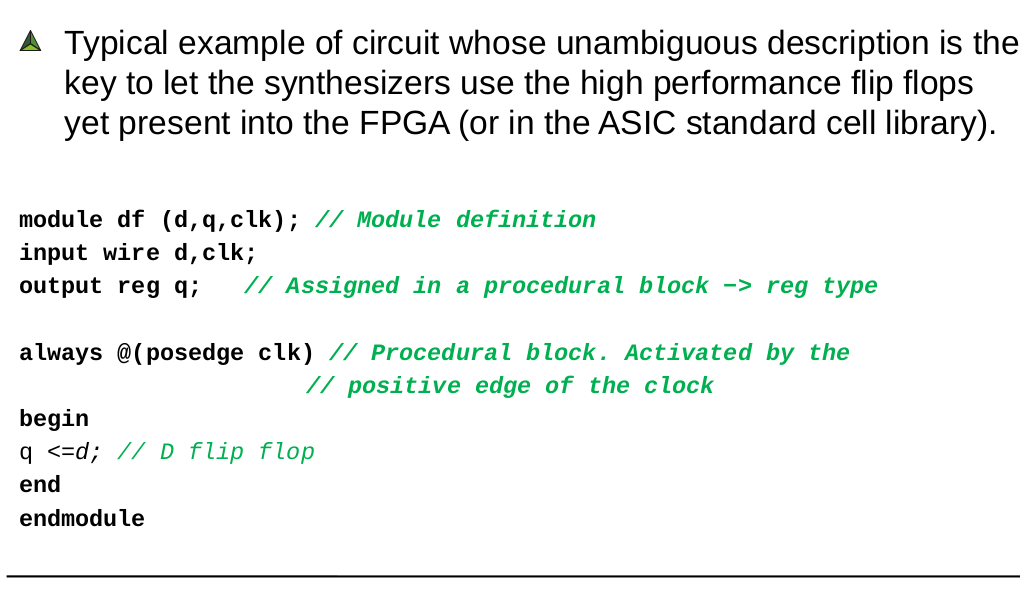
\includegraphics[width=0.5\linewidth]{img/chapt7img7.png}
        \end{figure}

    \section{Test bench}
        Il testbench non è un circuito ma un programma di test, quindi non ha né ingressi né uscite, quindi va dichiarato il module senza alcun argomento. Tutto quello che fa il testbench è pipare degli stimoli e verificare le uscite del circuito.
        \begin{figure}[h!]
            \centering
            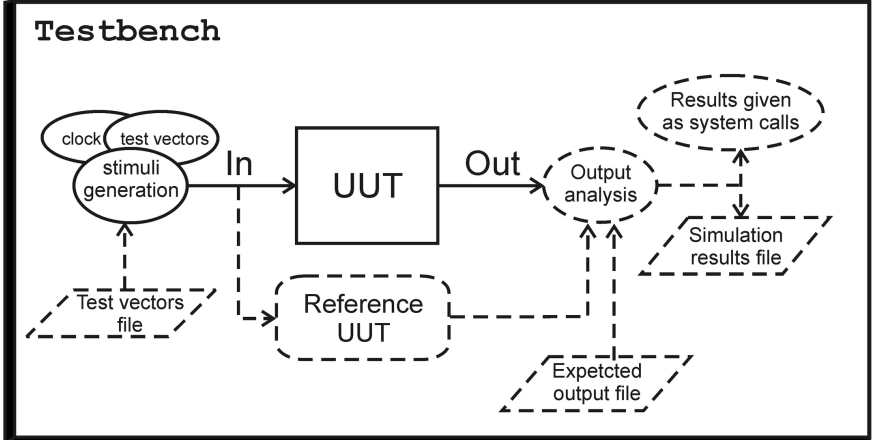
\includegraphics[width=0.5\linewidth]{img/chapt7img8.png}
        \end{figure}\\ Esempio testbench di un priority encoder 8:3
        \begin{figure}[h!]
            \centering
            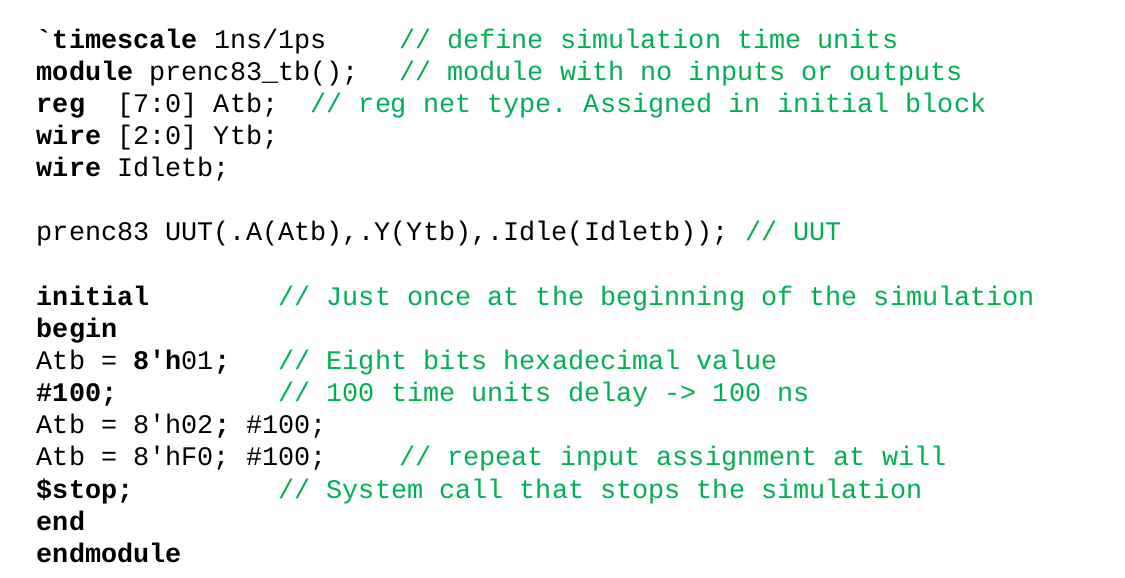
\includegraphics[width=0.5\linewidth]{img/chapt7img9.png}
        \end{figure}
        L'istruzione timescale da le unità di tempo di riferimento. ALl'interno dell'initial, \#100 si riferisce ad "aspetta 100 nanosecondi" perché il timescale ha il nanosecondo come unità di misura. La seconda unità di misura, il picosecondo, indica l'ultima cifra significativa da considerare per i valori del testbench. La sesta istruzione serve a collegare i segnali IO del circuito: i segnali collegati agli ingressi del testbench vanno definiti come reg, mentre quelli alle uscite come wire. Questa cosa è intuitiva perché i segnali d'ingresso devono stimolare i blocchi procedurali.

\chapter{Circuiti aritmetici}
    \section{Richiami sulla rappresentazione dei numeri}
        Un numero a virgola fissa senza segno si indica con la notazione:
        \begin{equation}
            U_{n,m}
        \end{equation}
        dove $n$ è la potenza di $2$ assegnata all'MSB della parte intera ed $m$ la potenza \textit{negativa} di $2$ assegnata all'LSB della parte frazionaria. Per esempio $U_{4,3}$ ha MSB di peso $2^{4}$ ed LSB di peso $2^{-3}$, dunque $U_{4,3} \in [0, 31.875]$. \\
        Per rappresentare invece numeri negativi a virgola fissa c'è il complemento a due. Un numero in complemento a due è indicato con:
        \begin{equation}
            Q_{n,m}
        \end{equation}
        dove $Q$ ricorda l'insieme dei numeri razionali. I parametri $n$ ed $m$ sono rispettivamente la potenza dell'MSB (numero negativo) e la potenza \textit{negativa} dell'LSB della parte frazionaria
        \begin{equation}
            Q_{n,m} = -2^{-n}A_{n+m} \ 2^{n-1}A_{n+m-1} \ \cdots 2^{-(m-1)}A_{1} \ 2^{-m}A_{0} 
        \end{equation}
        Per esempio
        \begin{equation}
            Q_{2, 0} = 1010 = -2
        \end{equation}
    \section{Rappresentazione in Verilog}
        Nel verilog, un wire può assumere il significato di un segnale o di un numero a seconda del contesto. Se per esempio $A$ è una stringa di $8$ bit che entra in un encoder, allora si starà trattando di un segnale, per esempio un vettore di priorità. Viceversa, se $A$ entra in un sommatore dobbiamo aspettarci che abbia valore aritmetico e non logico.
        \begin{figure}[h!]
            \centering
            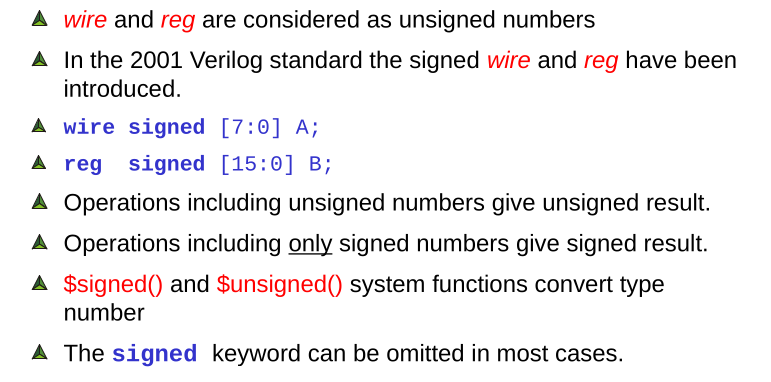
\includegraphics[width=0.75\linewidth]{img/chapt10img1.png}
        \end{figure} \\
    \section{Addizionatore binario}
        Un addizionatore binario è un circuito che ritorna la somma aritmetica degli ingressi. I bit di ingresso sono tre, i due operandi $A$ e $B$ ed il bit di riporto in entrata $C_{in}$. I bit di uscita sono la somma $S$, il segnale di overflow $OFL$ ed il riporto in uscita $C_{out}$. Il riporto in uscita può essere usato come l'$n+1$-esimo bit della somma ma non può essere usato per segnalare l'overflow (si può avere OFL con ambo i valori di Carry in uscita). \\
        Si possono ottenere addizionatori a $2n$ bit mettendone in cascata $2$ da $n$ bit e collegando il $C_{out}$ del primo al $C_{in}$ del secondo. I riporti in entrata degli addizionatori al primo stadio sono posti a massa.
        
        \begin{figure}[h!]
            \centering
            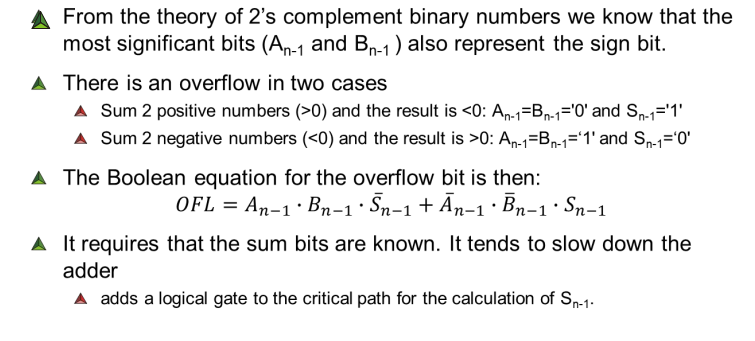
\includegraphics[width=0.75\linewidth]{img/chapt10img2.png}
        \end{figure}
        \begin{figure}[h!]
            \centering
            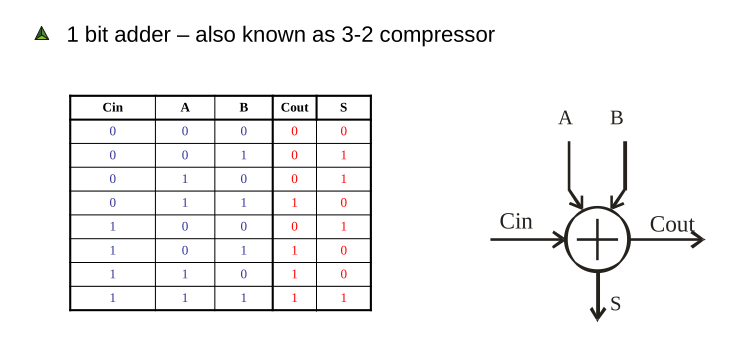
\includegraphics[width=0.75\linewidth]{img/chapt10img3.png}
        \end{figure}
        \newpage
        Se ci sono $n$ addizionatori in cascata, il tempo totale di delay tra l'ingresso del primo stadio e l'uscita dell'ultimo è pari a:
        \begin{figure}[h!]
            \centering
            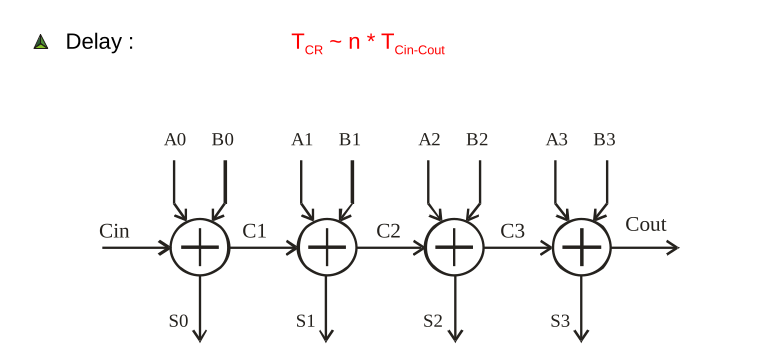
\includegraphics[width=0.75\linewidth]{img/chapt10img4.png}
        \end{figure}
        Un addiziontore del tipo di sopra è detto \textbf{carry ripple}, cioè a propagazione di riporto. Esso consta in $n$ addizionatori ad un bit, con l'uscita che viene presa in parallelo da ogni adder, collegato al precedente tramite il carry out. Questo è il circuito più semplice da realizzare per costruire un addizionatore, ha il minor consumo di potenza dissipata ma è anche il più lento con tempo pari a $T_{CR}$.
        \begin{figure}[h!]
            \centering
            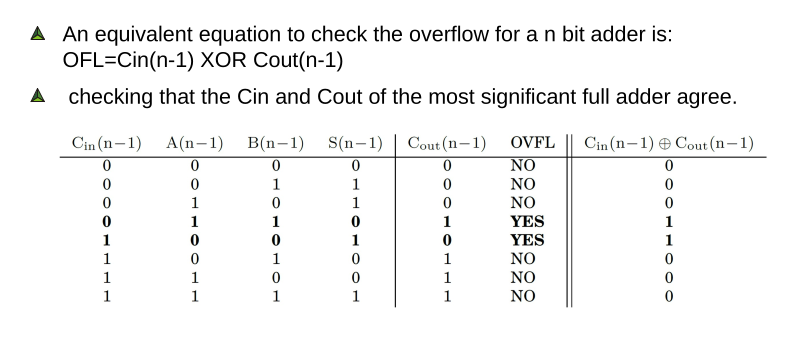
\includegraphics[width=0.75\linewidth]{img/Chapt10img5.png}
        \end{figure}
        \\ \\
        Per la sottrazione, il circuito è lo stesso del sommatore binario. La differenza $A-B$ è scritta come $A+(-B)$ dove $-B$ si ottiene negando $B$ bit per bit ed aggiungendo $1$, per esempio:
        \begin{equation}
            1110_{2} = (-2)_{10} \implies 0001_{2}+0001_{2} = 2
        \end{equation}
    \section{Topologie di addizionatori per FPGA}
        La topologia utilizzata per l'adder binario è quella a \textbf{carry ripple} con un piccolo fan-in. I blocchi logici delle moderne FPGA includono logica orientata alla propagazione del riporto, atta ad ottimizzare i collegamenti circuitali dei sommatori a carry ripple. Gli adder a carry ripple occupano molto poco spazio, dunque è possibile trovarne tantissimi anche nei più piccoli FPGA. \\ \\
        Negli adder carry ripple i bit di carry out dello stadio $n-1$ e di quello $n$ possono essere utilizzati per il check dell'overflow: se entrambi sono alti, allora c'è sicuro overflow:
        \begin{equation}
            OFL = C_{out, n-1} \oplus C_{out, n}
        \end{equation}
        Le prestazioni del circuito addizionatore si misurano in base al numero di Logic Element impiegati ed il ritardo di CR, entrambi funzione del numero di bit dell'addizionatore:
        \begin{figure}[h!]
            \centering
            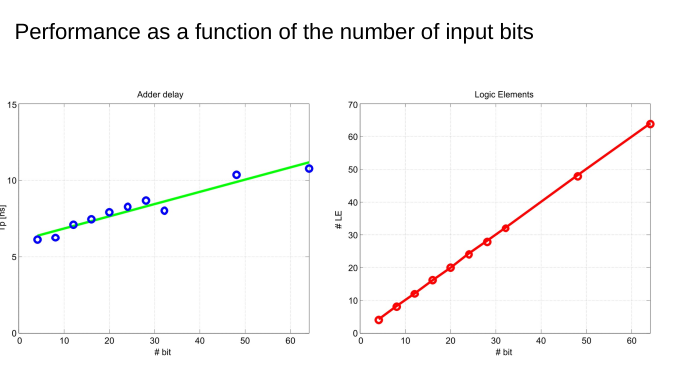
\includegraphics[width=0.75\linewidth]{img/chapt10img5.png}
        \end{figure}
    \section{Operazioni comuni}
        Molto spesso gli ingressi dei circuiti digitali sono numeri rappresentati in virgola fissa ma con un differente numero di bit o con la virgola in posizioni differenti. Le operazioni aritmetiche più comuni sono quelle che trasformano la rappresentazione di un numero eliminando o aggiungendo dei bit a destra o a sinistra della rappresentazione originaria. L’operazione sembra banale ma serve ad allineare la virgola di rappresentazioni diverse, a evitare e controllare i casi di overflow, a determinare la precisione di un’operazione aritmetica.
        \begin{figure}[h!]
            \centering
            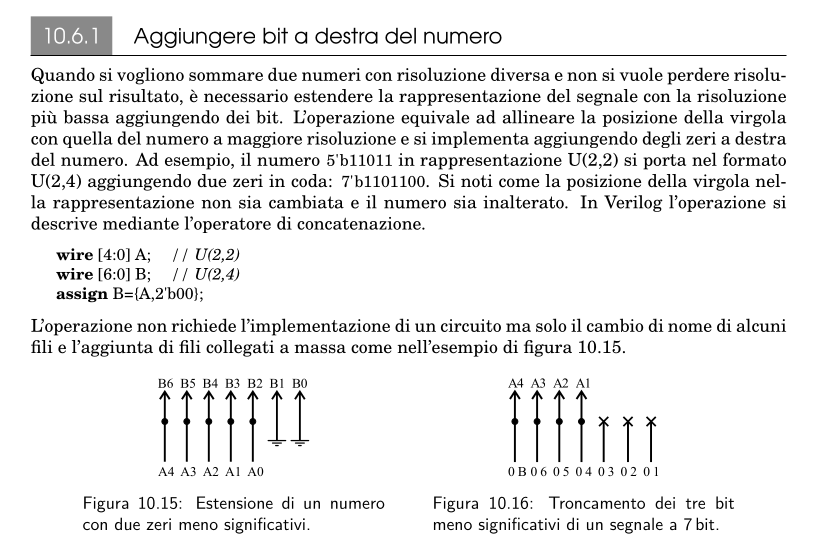
\includegraphics[width=0.65\linewidth]{img/chapt10img6.png}
        \end{figure} \newpage
        Talvolta si desidera ridurre la precisione di un numero per evitare che il numero di bit del
        risultato di un calcolo sia troppo grande o per rispettare i vincoli su un interfacciamento,
        e quindi bisogna eliminare i bit meno significativi del numero effettuando un’operazione di
        troncamento o di arrotondamento. Ad esempio, si utilizza il troncamento o l’arrotondamento
        se il risultato di un’operazione è su 16 bit mentre il registro nel quale bisogna memorizzare il risultato è da 8 bit.\\
        Il troncamento è il modo più semplice per eseguire l’operazione e consiste nello eliminare i
        bit che non si utilizzano. Un minimo di riflessione mostra che l’errore dovuto al troncamento è
        sempre dello stesso segno in quanto si azzerano sempre dei bit con peso positivo.
        Ritornando all’esempio in cui si eliminano 4 bit il cui LSB ha peso $2^{-5}$ , per effettuare
        l’operazione di arrotondamento bisogna sommare al numero da troncare il valore $2^{-2}$ prima
        di eliminare gli ultimi 4 bit. L’errore che si commette varia tra $-0.25$ (quando i 4 bit eliminati sono ‘1000’) a 0.2188 = $2^{-3} +2^{-4} +2^{-5}$ (quando i 4 bit eliminati valgono ‘0111’).
        \begin{figure}[h!]
            \centering
            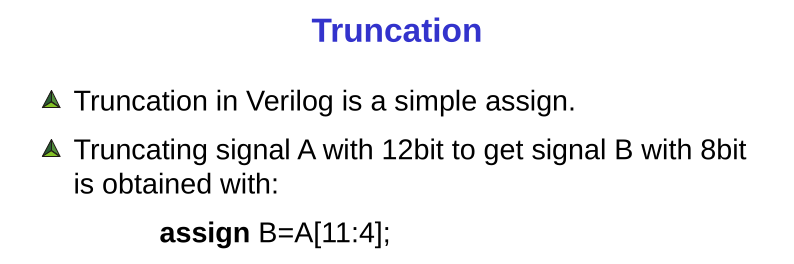
\includegraphics[width=0.65\linewidth]{img/chapt10img7.png}
        \end{figure}
        \begin{figure}[h!]
            \centering
            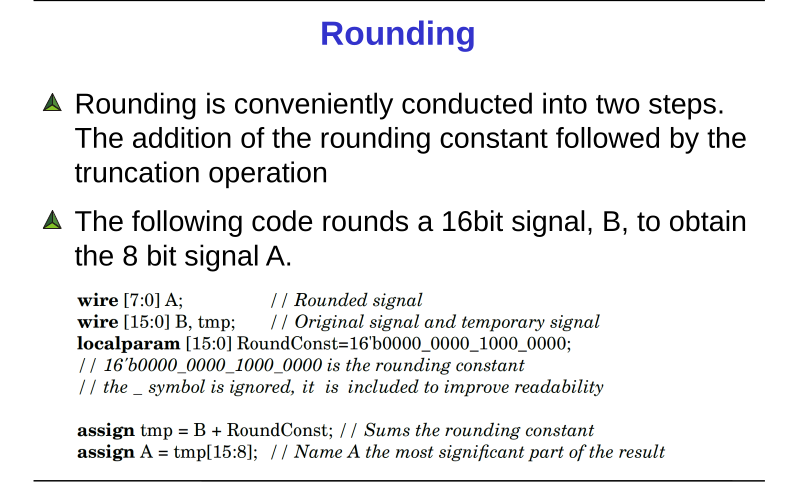
\includegraphics[width=0.65\linewidth]{img/chapt10img8.png}
        \end{figure}
        Per le operazioni di estensione:
        \begin{figure}[h!]
            \centering
            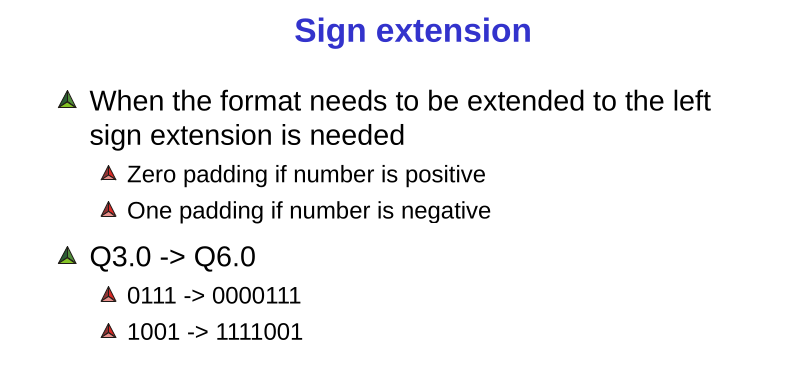
\includegraphics[width=0.5\linewidth]{img/chapt10img9.png}
        \end{figure}
        
    \section{Moltiplicazioni TBD}

\chapter{Circuiti sequenziali}
    \section{Introduzione}
        Circuiti che dipendono anche dal loro stato precedente. Non conviene 
        implementare un circuito sequenziale tramite logica combinatoria, per esempio 
        creando un flip flop dichiarando due inverter e poi collegandoli, ottenendo un 
        \textbf{loop combinatorio}, i quali non vengono risolti né in sintesi né in 
        simulazione. Utilizzeremo i blocchi procedurali con gli \textit{always} block. \\ \\
        \begin{figure}[h!]
            \centering
            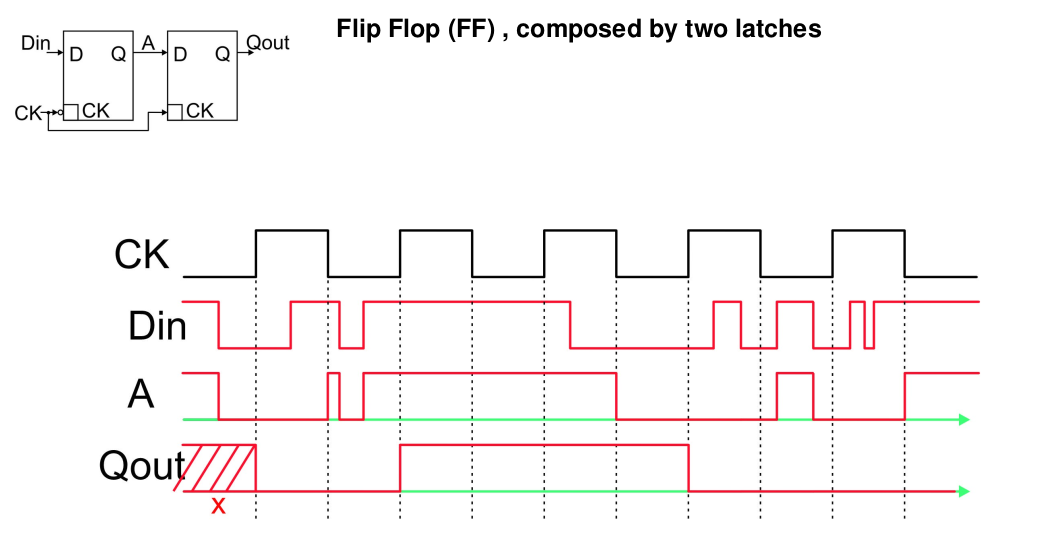
\includegraphics[width=0.5\linewidth]{img/Chapt11img1.png}
        \end{figure} \\
        Prima dell'accensione, il rumore elettronico determina lo stato di $Q_{out}$, il quale si stabilizza una volta iniziato il ciclo. Il flip flop varia il suo stato sul fronte di salita (o di discesa) del clock, ergo nel blocco procedurale ci sarà la sola dipendenza da CK\newpage
        \begin{figure}[h!]
            \centering
            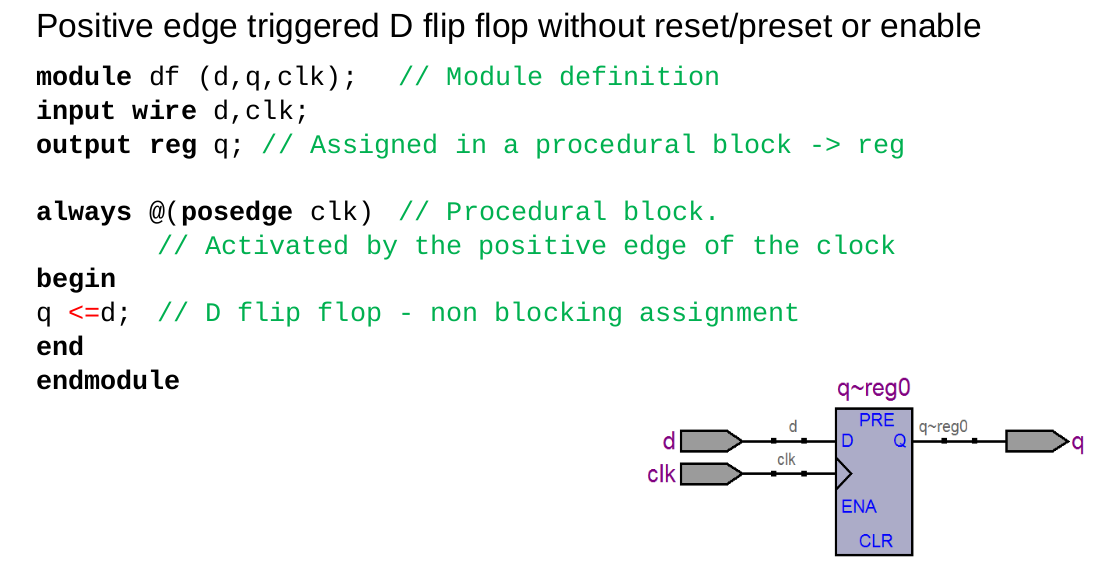
\includegraphics[width=0.75\linewidth]{img/chapt11img2.png}
        \end{figure} 
        Una versione più completa del FF introduce il segnale di Reset, che blocca l'uscita a zero. O lo si fa \textbf{sincrono} oppure \textbf{asincrono}, dunque due circuiti diversi. Nel primo caso, l'effetto del reset lo vedo solo appena il clock si alza, nell'altro caso l'uscita viene cambiata istantaneamente.
        \begin{figure}[h!]
            \centering
            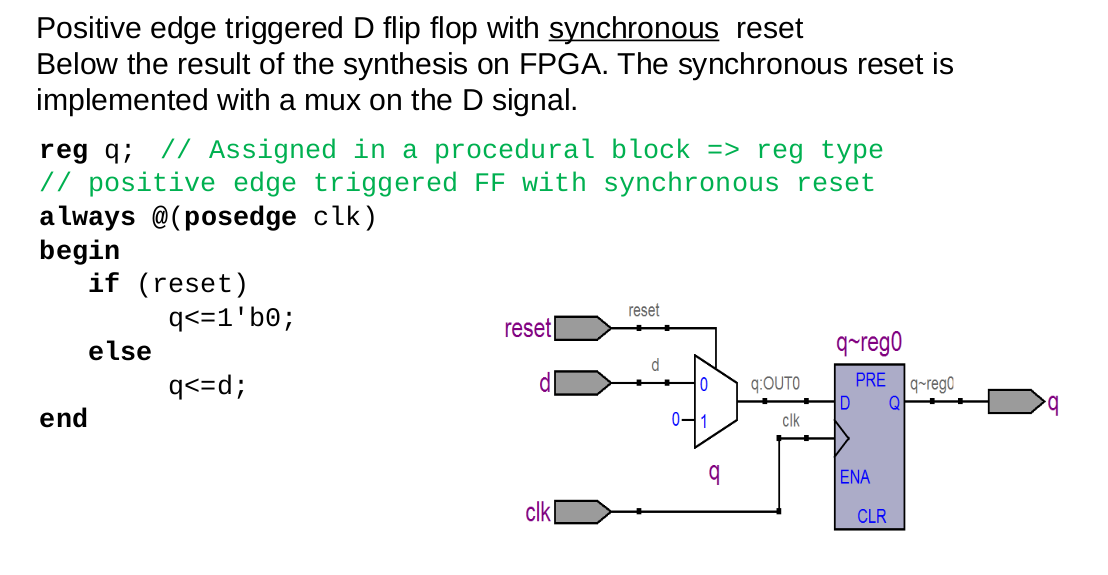
\includegraphics[width=0.75\linewidth]{img/chapt11img3.png}
        \end{figure}
        \begin{figure}[h!]
            \centering
            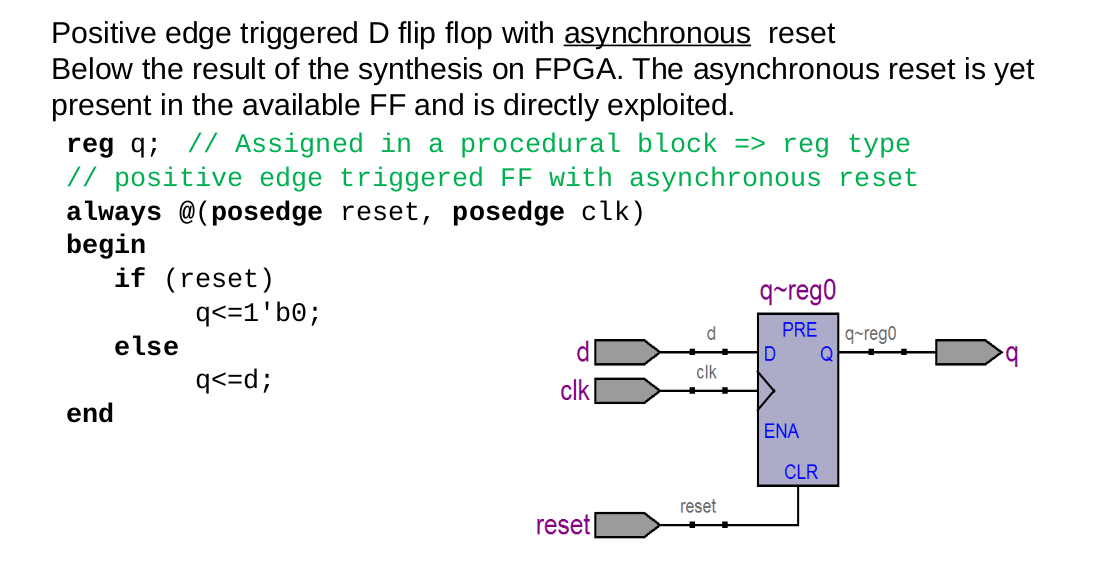
\includegraphics[width=0.75\linewidth]{img/chapt11img4.png}
        \end{figure} \newpage
        È importante usare la notazione blocking perché mettendo il minore uguale i due valori di $q$ commutano istantaneamente, mentre il non-blocking segna i valori e li cambia soltanto quando arriva all'istruzione end.
        \begin{figure}[h!]
            \centering
            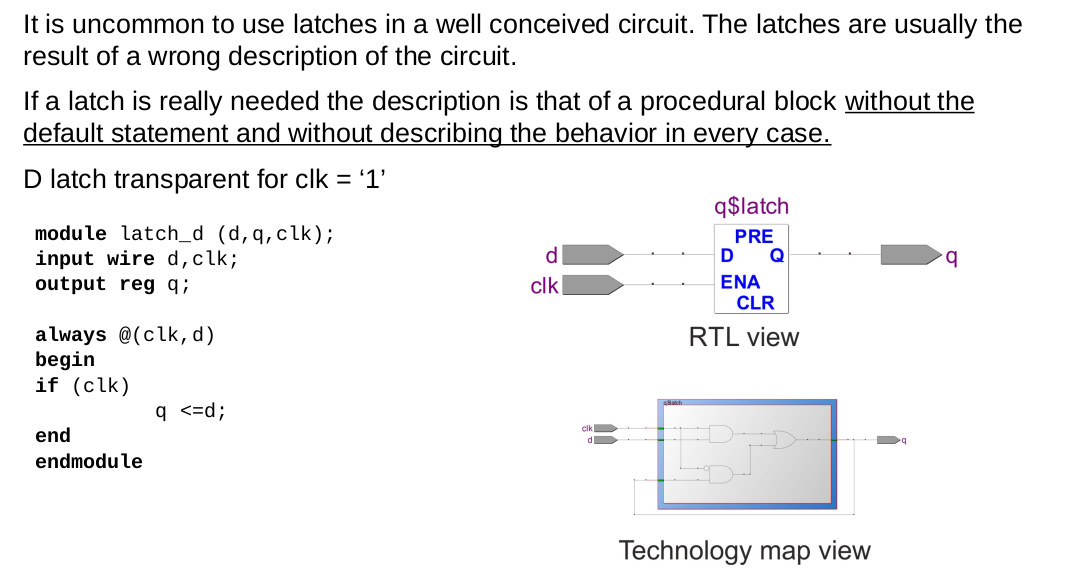
\includegraphics[width=0.75\linewidth]{img/Chapt11img5.png}
        \end{figure}
    \section{Test bench per circuiti sequenziali}
        A differenza del test bench per i combinatori, per i sequenziali bisogna implementare
        il clock in un blocco procedurale senza sensitivity list
        \begin{lstlisting}[language=Verilog]
localparam period=20; //Clock period is 20ns
    always
        begin
            CLKtb=1'b0;
            #(period/2.0); //2.0 is needed to obtain a real number
            CLKtb=1'b1;     
            #(period/2.0);
        end
        \end{lstlisting}
        Il test bench per un sequenziale si articola in tre momenti:
        \begin{itemize}
            \item La simulazione di un circuito sequenziale implica prima di tutto la fase di 
            reset. È buona pratica che, anche durante la fase di reset, tutti i segnali di input
            abbiano valore definito. Segue che la parte iniziale del test vector deve contenere
            le assegnazioni dei segnali di reset per tutti i segnali d'ingresso. 
            \item La seconda cosa da fare è disattivare il segnale di reset. Per ragioni di leggibilità,
            ogni volta che un segnale viene modificato, è conveniente ridefinire tutti i segnali di input
            e dunque è buona pratica riassegnare il valore di ogni segnale al momento della disabilitazione
            del segnale di reset.
            \item Durante il terzo momento il segnale di reset è disabilitato, dunque variano
            soltanto i segnali d'ingresso. È consigliato, sempre per ragioni di leggibilità, di evitare
            di riassegnare il valore del segnale di reset durante le rimanenti parti della simulazione, durante
            le quali ci limitiamo a cambiare soltanto il valore dei segnali d'ingresso.
        \end{itemize}
        Analizziamo un esempio di assegnazione corretta degli input e del segnale di reset. Il circuito
        d'esempio ha input $A$ e $B$ su 7 bit, un segnale di controllo $ctrl$ su 3 bit e i segnali di reset e 
        clear ($CLR$) espressi su singoli bit. È assunto che il segnale di cler sia attivo basso e che i 
        flip-flop siano sincronizzati sul fronte di salita del clock, generato dal codice scritto sopra.
        \begin{lstlisting}[language=Verilog]
initial
    begin
    //FASE 1: Reset attivo e valori di default per gli ingressi
    CLR = 1'b0; //Attivazione del reset
    A=y'b111_0000; B=7'b0; ctrl=3'b000; 
    // Assegna un valore ad ogni input. 
    //E' buona pratica non simulare con segnali indefiniti
    #(5*period) //Il reset dura cinque periodi di clock
    #(3*period/4.0); //Opzionale
                     //Le transizioni di input cominciano ad
                     //1/4 di periodo dopo il fronte di 
                     //attivazione, il tempo per il quale
                     //e' permesso il ritardo logico 
                     //combinatoriale e' 3/4 di periodo
    //FASE 2: disattivazione del reset
    CLR=1'b1; //Reset disattivato

    A=7'b000_0000; B=7'b0; ctrl=3'b000; 
    // non abbiamo modificato solo A bensi' anche quelli che 
    // non variano (buona pratica)
    #period;

    A=7'b000_0000; B=7'b0; ctrl=3'b001;
    #period;

    A=7'b000_0000; B=7'b101_1111; ctrl=3'b001;
    #period;

    A=7'b000_0100; B=7'b101_1111; ctrl=3'b000;
    #period;
    $stop; // sys-call per terminare la simulazione
end
        \end{lstlisting}
        \newpage
        \section{Altri circuiti sequenziali}
        \subsection{D-latch}
        Non è cosa comune utilizzare un latch in un cicuito ben progettato, perché di solito
        questi sono il risultato di una descrizione errata. Se un latch è veramente necessario,
        la descrizione è quella di un blocco procedurale senza il default statement e senza descrivere
        il comportamento in ogni caso. 
        \begin{figure}[h!]
            \center
            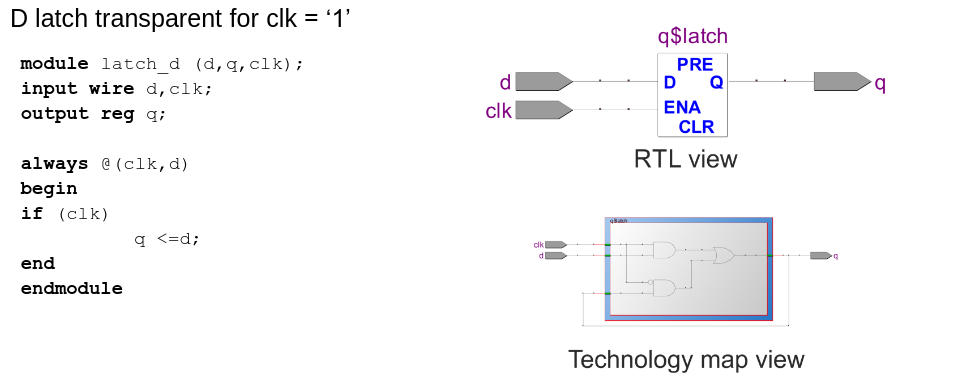
\includegraphics[width=0.75\linewidth]{img/chapt11img10.png}
        \end{figure}
        \subsection{Registri}
            Un registro è un insieme di flip-flop connessi in parallelo, dunque la relativa descrizione
            in verilog sarà un flip-flop che prende in ingresso un vettore dando in uscita un vettore:
            \begin{figure}[h!]
                \begin{center}
                    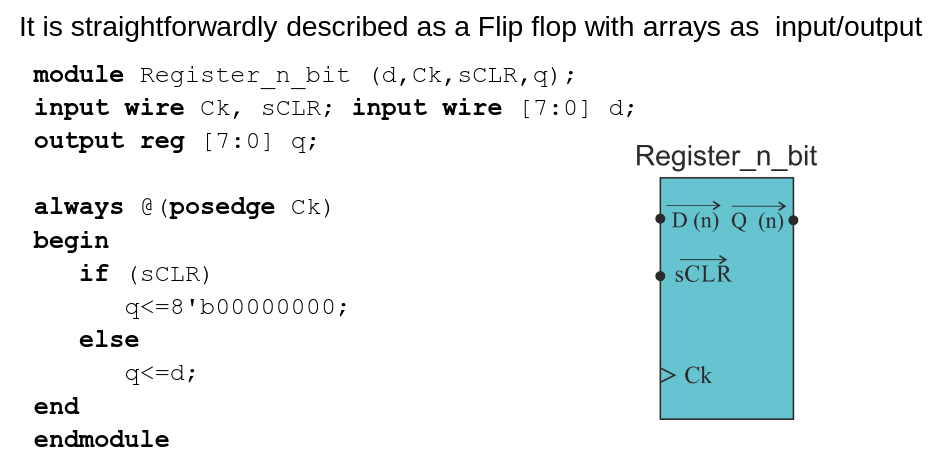
\includegraphics[width=0.75\linewidth]{img/chapt11img11.png}
                \end{center}
            \end{figure} \\
            La versione con l'enabler si ottiene con un blocco if: $en ? q<=d : q ;$
            \newpage
            \subsection{Registri a scorrimento}
            I registri a scorrimento (shift register) sono comunemente usati per conservare una sequenza di 
            dati in ingresso. Il circuito top level mostrato in figura ha un bit d'ingresso ed
            $n$ "taps", cioè dati conservati.
            \begin{figure}[h!]
                \center 
                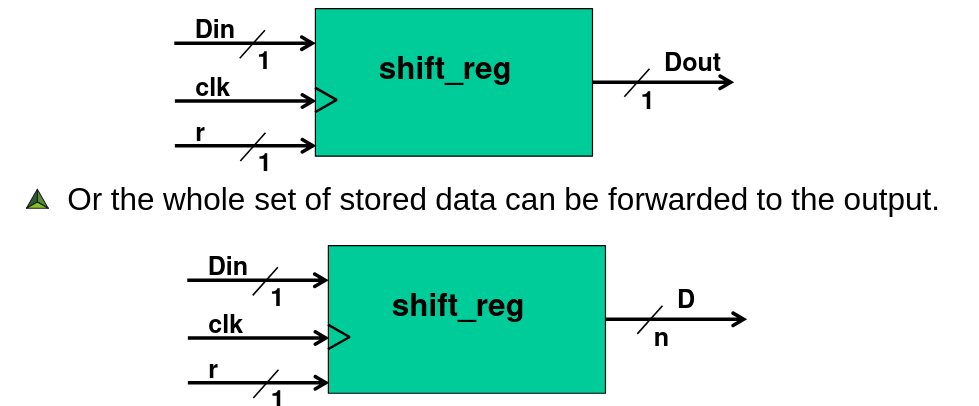
\includegraphics[width=0.75\linewidth]{img/chapt11img12.png}
            \end{figure}
            Un utilizzo comune degli shift register è quello di ritardare un segnale di $n$ colpi di clock,
            dove $n$ è il numero di tap del registro.
            \begin{figure}[h!]
                \center 
                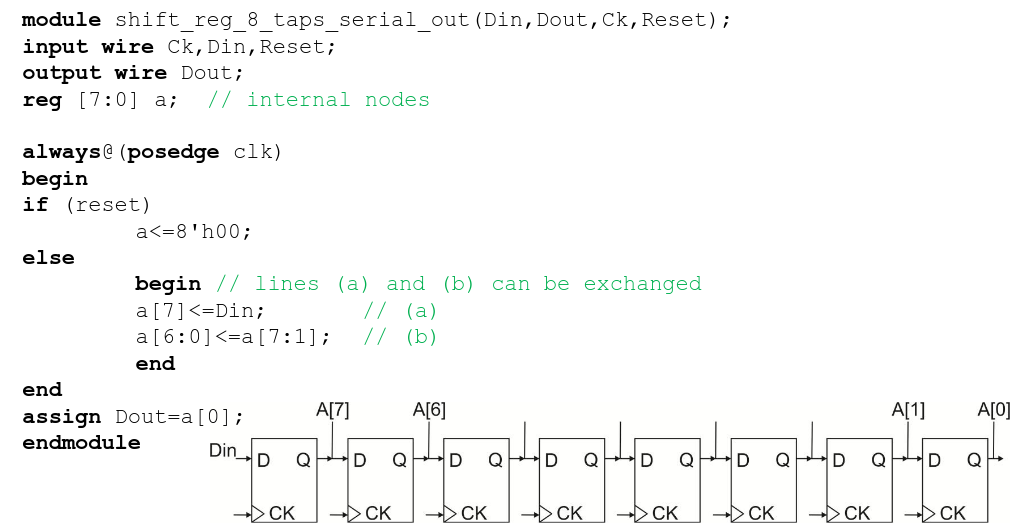
\includegraphics[width=0.75\linewidth]{img/chapt11img13.png}
            \end{figure}
            \newpage
            L'implementazione di sopra si può generalizzare al caso di uno shift register con
            ingressi ad $m$ bit. Di seguito è riportato come esempio l'implementazione di un registro
            a scorrimento con ingresso a $16$ bit ed $8$ tap.
            \begin{figure}[h!]
                \center
                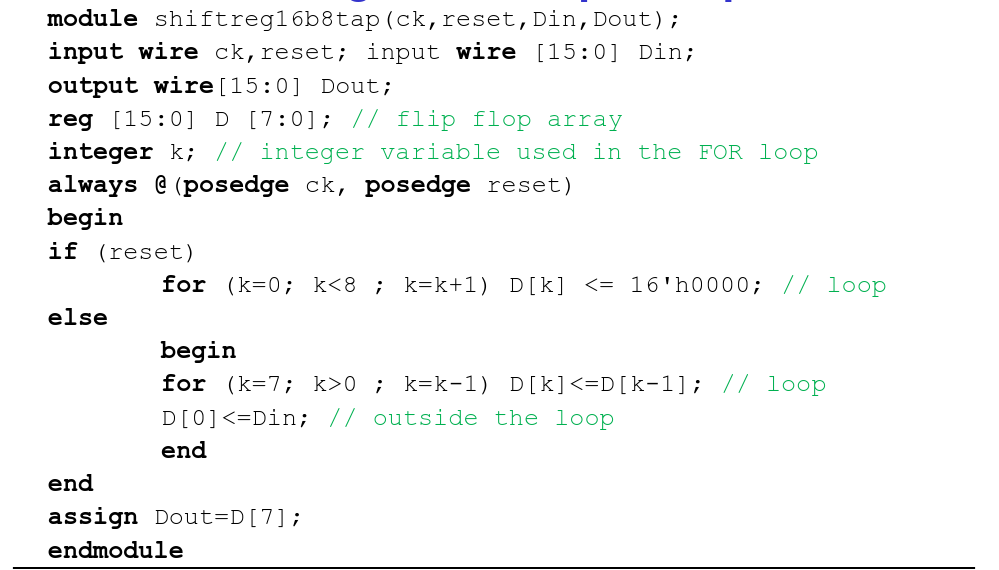
\includegraphics[width=0.75\linewidth]{img/chapt11img14.png}
            \end{figure}
    \subsection{Contatori}
            I contatori sono parecchio comuni nei circuiti digitali. Sono usati per 
            sincronizzare differenti sezioni in termini di numero di colpi di clock.
            Trovano svariate applicazioni: dividere bit in byte/word, determinare i bit di parità,
            permettere il time delay di segnali
            Quando non specificato altrimenti dal segnale di controllo, un contatore può contare
            da $0$ a $2^{n}-1$.
            \\ La struttura basica di un contatore è quella di un accumulatore, il quale 
            a sua volta è composto da un addizionatore e da un registro. Contatori più complessi utilizzano
            segnali per contare fino a valori diversi da $2^{n}-1$, generati aggiungendo strutture MUX.
            \begin{figure}[h!]
                \center  
                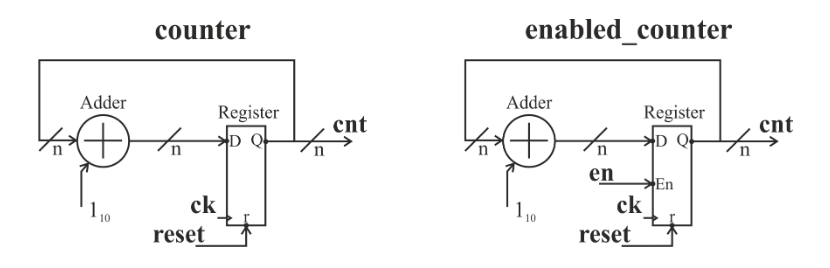
\includegraphics[width=0.75\linewidth]{img/chapt11img15.png}
            \end{figure}
            \begin{figure}[h!]
                \center  
                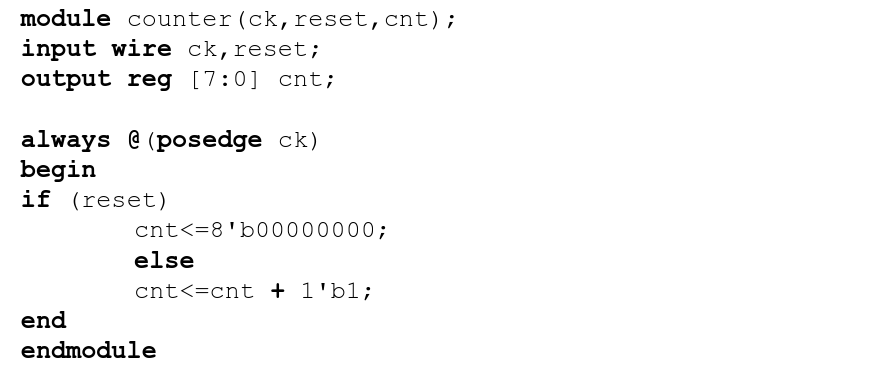
\includegraphics[width=0.55\linewidth]{img/chapt11img16.png}
            \end{figure} \newpage
    Per implementare una versione con limite superiore diverso da $2^{n}-1$, basta aggiungere
    un altro blocco if che resetta il contatore una volta raggiunto tale limite.
    \subsection{Accumulatori}
        È come un contatore, solo che al posto di incrementare l'output di uno ad ogni
        colpo di clock, incrementa l'output aggiungendo il valore provvisto dall'ingresso.
    \subsection{Serial adder}
        Un addizionatore carry ripple è composto da full adder in cascata ed esegue la somma
        in un singolo colpo di clock. Se si ammette che tale operazione possa essere fatta in più di un
        colpo di clock, si può pensare ad una topologia che utilizza gli stessi full adder per
        fare una singola somma, risparmiando una notevole quantità di area. Per fare ciò bisogna
        passare i bit degli addendi uno alla volta, dunque un adder seriale prende dati d'ingresso da due
        registri e li somma. Il risultato va in un registro di uscita e viene shiftato di una posizione ad ogni somma
        che viene fatta. Il carry out va in un flip-flop e viene multiplexato con un segnale newop (nuova operazione):
        se si sta ancora facendo l'operazione, viene sommato il resto, altrimenti viene settato il carry in a zero e si riparte
        da capo.
        \begin{figure}[h!]
            \center
            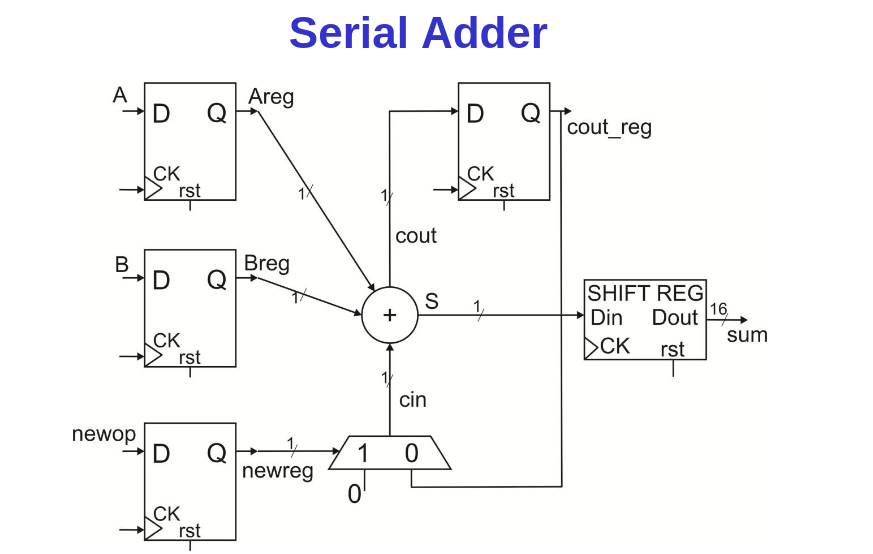
\includegraphics[width=0.75\linewidth]{img/chapt11img17.png}
        \end{figure}
    \chapter{Temporizzazione di circuiti sequenziali}
    \section{Circuiti sincroni e asincroni}
        I circuiti sincroni sono temporizzati tutti con lo stesso clock, mentre quelli asincroni no.
        \begin{figure}[h!]
            \centering
            \includegraphics[width=0.75\linewidth]{img/chapt12img1.png}
        \end{figure}
        \begin{figure}[h!]
            \centering
            \includegraphics[width=0.75\linewidth]{img/chap12img2.png}
        \end{figure}
        Il 99\% dei circuiti digitali sono sincroni.
    \section{Timing dei Flip-Flop}
        I flip flop si comportano come circuiti di campionamento. Il campionamento ideale
        ed il cambiamento istantaneo del segnale non è possibile. I parametri che determinano
        il comportamento di timing del flip flop sono:
        \begin{itemize}
            \item Il tempo di setup $t_{s}$, intervallo di tempo prima del fronte del clock
            in cui il dato deve essere stabile 
            \item Il tempo di hold $t_{h}$, intervallo di tempo dopo il fronte di clock in cui il dato deve essere stabile
            \item Il tempo di ritardo del clock a $q$ $t_{q}$, il ritardo di propagazione fra il fronte attivo del clock
            e il segnale $q$, cioè quanto ci mette il FF a variare la sua uscita.
        \end{itemize}
        Notare che $t_{q}$ e $t_{h}$ rappresentano due cose diverse: il primo è il tempo necessario
        affinché lo stato si propaghi in uscita, mentre il secondo il tempo necessario per evitare fluttuazioni
        di stato del FF prima di aver finito di caricare le capacità d'ingresso del circuito a valle.
        Vediamo un esempio di timing corretto e scorretto e vediamo in cosa differiscono.
        Partiamo dal diagramma temporale di un flip-flop e analizziamone i vincoli di setup
        \begin{figure}[h!]
            \center  
            \includegraphics[width=0.75\linewidth]{img/chapt12img3.png}
        \end{figure} \\
        Nello schema $y$ è l'ingresso e $x$ l'uscita\footnote{Scelta peculiare}
        L'intervallo di tempo $T_{C,max}$ è il \textbf{ritardo combinatoriale massimo} e dipende
        dal percorso del segnale e deal numero di porte logiche attraversate dal circuito combinatorio.
        Come da definizione, il tempo impiegato da $q$ (in questo caso chiamato $x$) per commutare è proprio $t_{q}$
        \\ \\
        Facciamo un quadro di ciò che sta accadendo in figura: l'ingresso $y$ varie e dopo $t_{q}$ secondi
        varia anche lo stato $Q$ del flip-flop, rappresentato dal segnale $x$ in figura. Poi il segnale $x$ entra 
        nella logica combinatoria e dopo un tempo combinatoriale che è al massimo $T_{C,max}$ questo esce. Il dato 
        in uscita dalla logica combinatoria deve essere stabile almeno $t_{s}$ secondi prima del prossimo fronte attivo 
        (in salita nel nostro caso). \\
        Questo ci porta a definire il primo dei due vincoli, quello di \textbf{setup}. Il vincolo di setup 
        si calcola fra i due fronti attivi del clock ed è riferito a due circuiti che si passano il dato. Quello che
        eroga il dato è detto "launching" mentre quello che lo prende in ingresso è il "capturing". Nel
        disegno di sopra il FF è al tempo stesso launching e capturing, perché lancia il dato e se lo riprende dopo che questo
        è uscito dalla logica combinatoria. Se $t=0$ corrisponde all'istante in cui c'è il primo fronte attivo e $T$ quello in cui 
        c'è il secondo, il vincolo di setup è dato da:
        \begin{equation}
            T>t_{q}+T_{c,max}+t_{s}
        \end{equation}
        questo perché dopo il fronte il dato ci mette $t_{q}+T_{c,max}$ secondi ad uscire dalla logica combinatoria e 
        deve essere pronto almeno $t_{s}$ secondi prima del prossimo fronte, dunque l'intervallo $T$ deve essere abbastanza largo 
        per soddisfare questo margine. La differenza fra $T$ ed il valore minimo di $T$ per cui il vincolo di setup è verificato e 
        è detta \textbf{slack}:
        \begin{equation}
            \textrm{T}=T_{C,max}+t_{q}+t_{s}+\textrm{Slack}\implies \textrm{Slack}=T-T_{c,max}-t_{q}-t_{s}
        \end{equation}
        Dunque il vincolo di setup da un limite superiore alla frequenza di clock.
        \\ \\
        Passiamo ora al vincolo di \textbf{hold}, che si applica su un singolo fronte di clock. Il vincolo di hold è 
        dato in sostanza dal tempo che serve al flip flop di far propagare il dato che ha già all'interno mentre arriva quello nuovo. In altre 
        parole, è un vincolo su quanto lento deve andare il segnale in ingresso affinché lo stato precedente sia propagato senza fastidi.
        \begin{figure}[h!]
            \center   
            \includegraphics[width=0.5\linewidth]{img/chapt12img4.png}
        \end{figure} \\
        Allora partendo dal fronte di salita devono passare $t_{h}$ secondi dati dal tempo di hold prima che il 
        dato nuovo arrivi. Tale dato impiega, per arrivare, un tempo minimo dato da $t_{q}+T_{c,min}$, dunque deve verificarsi:
        \begin{equation}
            T_{c,min}+t_{q}>t_{h}
        \end{equation}
        che come dicevamo prima è una condizione di "lentezza" per i ldato in ingresso.
        Anche qui si può definire uno slack:
        \begin{equation}
            T_{c,min}+t_{q}=t_{h}+\textrm{Slack}
        \end{equation}
        Per il vincolo di setup il progettista può procedere ad abbassare la frequenza, mentre per quello di hold si hanno 
        le mani legate dalla tecnologia, perchè $t_{q}$ e $t_{h}$ sono caratteristiche del FF e $T_{c,min}$ della rete combinatoria, dunque 
        a priori vanno scelti dei componenti che abbiano tempistiche compatibili. In ogni caso, un FF ben costruito ha il tempo di 
        propagazione dello stato $t_{q}$ maggiore di quello di hold $t_{h}$. \\ \\
        Per fare il timing di tutto il sistema e decidere la frequenza massima da utilizzare, si studia caso per caso 
        il vincolo di setup e di hold e si raccolgono i valori di slack: il più basso determina la frequenza massima di lavoro. Se almeno uno 
        degli slack ha valore negativo bisogna allungare il periodo di clock, abbassando la frequenza.
        \begin{figure}[h!]
            \center  
            \includegraphics[width=0.75\linewidth]{img/chapt12img5.png}
        \end{figure}
        Le espressioni riportate in figura discendono dalla banale generalizzazione di quello di cui abbiamo parlato sopra. Se 
        prendiamo ad esempio il pezzo di percorso $1 \to 3$, ci si rende conto che $1$ lancia e $3$ cattura, quindi il vincolo 
        di setup deve tenere conto del tempo $t_{q1}$ del lanciatore e del tempo di setup $t_{s3}$ del catturatore, assieme al tempo combinatoriale 
        massimo del blocco $A$. Per il vincolo di hold, è $t_{h3}$ che pone il vincolo per il dato in ingresso, che per arrivare 
        da $1$ a $3$ impiega $t_{c,min}+t_{q1}$.
        \\ \\
        A chiusura di questa sezione parliamo del Clock skew e gli effetti che questo ha sui vincoli di timing.
        Finora abbiamo considerato circuiti che hanno tutti lo stesso periodo di clock, ma possiamo pensare di inserire dei 
        blocchi di ritardo del segnale per dare una versione ritardata del clock in ingresso ad alcuni blocchi del circuito, come 
        in figura:
        \begin{figure}[h!]
            \center  
            \includegraphics[width=0.6\linewidth]{img/chapt12img2.png}
        \end{figure} \\
        Il blocco di ritardo posticipa di $\Delta t$ l'inizio dell'intervallo di setup del FF catturatore a destra, 
        ma al tempo stesso ne riduce quello di hold della stessa quantità:
        \begin{figure}[h!]
            \center  
            \includegraphics[width=0.5\linewidth]{img/chapt12img6.png}
        \end{figure}
        Se ricalcoliamo il vincolo di setup otteniamo, ipotizzando che i due flip flop siano uguali:
        \begin{equation}
                T>t_{q}+T_{c, max}+(t_{s}+\Delta t)
        \end{equation}
        Ma al tempo stesso, il vincolo di hold diviene:
        \begin{equation}
            t_{q}+T_{c,min}>t_{h}+\Delta t
        \end{equation}
        questo perché traslando il clock si trasla anche l'istante per cui il tempo di hold è soddisfatto, visto che come 
        riferimento $t_{h}$ prende proprio il fronte attivo del clock. In sintesi, il clock skew può essere una risorsa nel caso
        si abbia molto margine con uno dei due parametri: per esepmio, lo slack del tempo di setup è molto ampio e invece di alzare la frequenza 
        si vuole puntare sulla robustezza, allora si mette un blocco di ritardo da qualche parte per "donare" tempo di slack al vincolo di hold.
        \newpage
        \section{Applicazione al design di FPGA}
        \subsection*{Cenni agli alberi di clock}
            Di Flip-Flop all'interno di in un circuito digitale ce ne sono milioni, ragion per la quale pensare 
            che il clock arrivi in sincronia ovunque è una brutale idealizzazione. Questo è dovuto, oltre al carico capacitivo 
            non trascurabile di tali circuiti, anche alla lunghezza delle piste fra l'origine del clock e i flip-flop. Per ovviare a 
            questa cosa, si è pensato di collegare i flip flop ad albero, interponendo dei buffer ogni tot sezioni. Le strutture di questi 
            alberi sono calcolate tramite algoritmi appositi, fatti girare da programmi dedicati. Si ottiene una maggior omogeneità del clock skew 
            in giro per il circuito, pagando però un grosso ritardo $T_{clk, buf}$ (legato ai buffer) tra l'origine dell'albero e i suoi punti capillari:
            \begin{figure}[h!]
                \center  
                \includegraphics[width=0.6\linewidth]{img/chapt12img7.png}
            \end{figure}
        \subsection*{Pad to pad hold time}
            Per chi progetta su FPGA il clock tree non è una preoccupazione. Il progettista deve occuparsi però 
            della scelta opportuna della frequenza di lavoro, perché deve soddisfare sia i tempi di hold e di setup all'interno del circuito 
            che quelli dovuti all'interazione con circuiteria esterna, che lavora con tempi generalmente diversi. \\
            Fino ad ora abbiamo ignorato la circuiteria legata al clock e assunto che le equazioni sui vincoli potessero 
            essere ricavate dai tempi dei segnali in ingresso al flip-flop. Questa assunzione non è sempre corretta perché bisogna fare riferimento 
            ai punti di circuiteria accessibili al progettista, perché è lì che si possono fare le misure per i vincoli.
            Nell'immagine che segue confrontiamo una situazione ideale con una reale, che tiene conto del ritardo  
             dal buffer del clock che fornisce il ritardo $T_{clk, buf}$. Il ritardo di linea è dato da $T_{1}$ e $T_{2}$. Possiamo arbitrariamente inserire
            un blocco "Delay" di ritardo sulla linea dati:
        \begin{figure}[h!]
            \center  
            \includegraphics[width=0.75\linewidth]{img/chapt12img8.png}
        \end{figure} \\
        Sotto queste condizioni la condizione di hold diventa:
        \begin{equation}
            t_{q, 1}+T_{c,min}+T_{1}+\textrm{Delay}\geq T_{2}+T_{clk,buf}+t_{h2}
        \end{equation} \\
        questo perché al tempo di transizione di stato $t_{q1}$ va aggiunto il ritardo di linea, il ritardo del dato (blocco inserito da noi)
        e quello minimo della rete combinatoria. La somma di questi tre contributi deve essere maggiore del tempo di hold,
        a cui però va aggiunto il ritardo di clock e quello della rete di sotto $T_{2}$.
        Assumendo $T_{1}=T_{2}$ e che i flip flop siano uguali si ottiene una relazione indicativa ma abbastanza accurata per il vincolo di hold:
        \begin{equation}
            t_{q}+T_{c,min}+\textrm{Delay} \geq T_{clk, buf}+t_{h}
        \end{equation}
        Il blocco di delay è arbitrario e lo si può scegliere in modo da essere comparabile al ritardo dovuto al buffer, ottenendo:
        \begin{equation}
            t_{q}+T_{c,min} \geq t_{h}
        \end{equation}
        \subsection*{Aggiunta di un Delay Locked Loop}
        La situazione può essere migliorata ulteriormente per quanto concerne il tempo di hold 
        aggiungendo un DLL (Delay Locked Loop) come nello schema in figura:
        \begin{figure}[h!]
            \center  
            \includegraphics[width=0.75\linewidth]{img/chapt12img9.png}
        \end{figure}
        In questo caso non abbiamo inserito il blocco di delay, bensì un blocco DLL retroazionato che stabilizza il ritardo
        un ritardo sulla linea di clock dato da: $T_{DLL}=T_{2}-T_{clk,buf}$. Assumendo sempre $T_{2} = T_{1} = T$ e 
        FF uguali, il vincolo sul tempo di hold diventa:
        \begin{equation}
            t_{q}+T_{c,min}+T_{1} \geq t_{h}+T_{2}+(T_{2}-T_{clk, buf})+T_{clk,buf}
        \end{equation}
        \begin{equation}
            \implies t_{q}+T_{c,min} \geq T+t_{h}
        \end{equation}
        Poiché il clock è periodico di $T$, la condizione si riduce a:
        \begin{equation}
            t_{q}+T_{c,min} \geq t_{h}
        \end{equation}
        In altre parole, tramite il circuito di clock management basato su DLL possiamo far rispettare il vincolo 
        di hold per due circuiti diversi che comunicano fra di loro in modo stabile e configurabile per diversi valori di ritardo 
        di linea di clock.
    \section*{Management tramite clock gating}
        La terza e ultima tecnica che vediamo per la gestione dei vincoli di timing è basata 
        sulla tecnica del clock gating. Per clock gating si ci riferisce a quelle tecniche che utilizzano 
        logica combinatoria per sincronizzare solo alcune parti del circuito. Anni fa, utilizzare 
        il clock gating era un casino a causa degli ulteriori ritardi introdotti dalla logica circuitale e dal pericolo
        di generare glitch. Al giorno d'oggi sono indispensabili per azzerare la frequenza di lavoro delle parti inutilizzate del circuito
        e sincronizzare i ritardi. La loro robustezza è cresciuta molto grazie ai software che tengono conto dei ritardi nativi 
        di questi elementi circuitali. Lo schema a cui facciamo riferimento è il seguente:
        \begin{figure}[h!]
            \center  
            \includegraphics[width=0.75\linewidth]{img/chapt12img10.png}
        \end{figure} \\
        Si vede già dallo schema che il clock gating infastidisce il tempo di hold, perché introdurrà un 
        ritardo di natura combinatoria al clock che aumenterà il tempo di hold totale. Se partiamo dall'inizio, 
        grazie all'albero di clock i due segnali $Ck_{1}$ e $Ck_{2}$ sono sincronizzati, quindi il paragone va fatto a 
        partire da quei due punti li. Il tempo che ci mette il dato lanciato ad arrivare è $t_{q}+T_{c,min}$, mentre quello 
        dato dall'hold sarà $t_{h}+T_{GATING}$. In definitiva:
        \begin{equation}
            t_{q}+T_{c,min} \geq T_{GATING}+t_{h} = t_{h,eff}
        \end{equation} 
        dove $t_{h,eff}=T_{GATING}+t_{h}$ è il tempo di hold "efficace". Il gating incide anche sul tempo di 
        setup, che assume la forma seguente:
        \begin{equation}
            T>t_{q}+T_{c,max}+t_{s}-T_{GATING} \implies T>t_{q}+T_{c,max}+t_{s,eff}
        \end{equation}
        che ha parecchio senso se si tiene conto del fatto che se peggiora l'hold a causa di
        un ritardo del clock migliora il setup, come abbiamo visto in precedenza.
    \newpage
    \section{Timing analysis in vivado}
    Per il timing analysis in vivado, dobbiamo creare una risorsa .xdc per gestire il clock.
    In questo file dobbiamo essenzialmente dire a vivado di associare un clock virtuale all'ingresso
    di clock del nostro programma, così che possa verificare se i vincoli sono rispettati:
    \begin{figure}[h!]
        \center  
        \includegraphics[width=0.7\linewidth]{img/chapt12img11.png}
    \end{figure} \\
    Questo comando cosa fa? Crea un oggetto clock $(create \_ clock)$, lo aggiunge se non esiste già (-add)
    e gli da il nome di $sys \_ clk \_ pin \ \ (-name sys\_clk\_pin)$, con periodo 10.00timescale (-period 10.00) con
    duty cycle del 50\% (-waveform \{0 5\}) assegnandolo al segnale di clk  dichiarato nel file verilog (il "programma"),
    tramite il comando $[get\_ports\{clk\}]$.

    Concludiamo con un esempio. Consideriamo una situazione reale, dove ci sono due 
    registri che comunicano un ingresso alla nostra IP (Intellectual Property, in pratica il circuito), che li 
    elabora e li risputa fuori in pasto ad un altro circuito.
    \begin{figure}[h!]
        \center  
        \includegraphics[width=0.6\linewidth]{img/chapt12img12.png}
    \end{figure} \\
    Dobbiamo tenere conto dei valori minimi e massimi di ritardo per i segnali di ingresso (A, B e il reset)
    e i valori minimi e massimi per quelli di uscita (P nel nostro caso). Allora il file .xdc si espande come segue:
    \begin{figure}[h!]
        \center 
        \includegraphics[width=0.75\linewidth]{img/chapt12img13.png}
    \end{figure}
\chapter{Dissipazione di potenza negli FPGA}
    \section{Introduzione}
        La dissipazione di potenza è uno dei parametri più importanti da considerare nei circuiti 
        digitali, perché costituisce un limite. Perché, in particolare, dovrebbe importarci di gestire 
        la dissipazione di potenza?
        \begin{itemize}
            \item \textbf{Per l'utente mobile}: cellulari, fotocamere e qualsiasi altro device mobile ha una batteria,
            la quale si scarica molto più velocemente se la quantità di potenza dissipata non è ottimizzata
            \item \textbf{Potenza computazionale}: i circuiti caldi hanno problemi di saturazione di frequenza di lavoro e power throttling 
            (letteralmente "strozzatura della potenza"), che ne riduce drasticamente le prestazioni 
            \item \textbf{Inquinamento}: più consumi porta a più sprechi 
        \end{itemize}
    Per il progettista, i punti 1 e 3 pongono dei limiti alla potenza media consumata dal circuito, mentre 
    il punto due alla potenza di picco. Ridurre la potenza di picco consente di ridurre i costi e le dimensioni
    delle infrastrutture di raffreddamento nei chip che, a fronte della riduzione di potenza media, lavoreranno a temperature
    più basse. La riduzione della potenza media permette anche di avere alimentatori più piccoli e compatti. Tutto ciò 
    migliora di gran lunga l'affidabilità del sistema. 
    \\ \\
    \section{Calcolo e stima della potenza}
        Come sappiamo, in un circuito digitale distinguiamo la potenza dissipata statica, legata 
        soprattutto alle perdite, da quella dinamica, legata all'attività del circuito. 
        \\ Per quanto concerne la potenza dissipata statica, questa è data dal prodotto fra
        la corrente $I_{DD}$ che il circuito assorbe dall'alimentazione e l'alimentazione $V_{DD}$.
        Poiché la corrente può dipendere dallo stato del sistema, se $P(\cdot)$ è la probabilità di stare 
        in un certo stato:
        \begin{equation}
            P_{s} = V_{DD}[P(V_{O}=V_{OL})I_{DD}(V_{0}=V_{OL})+P(V_{O}=V_{OH})I_{DD}(V_{O}=V_{OH})]
        \end{equation}
        Mentre quella dinamica è:
        \begin{equation}
            P_{D}= \alpha f_{clk}CV_{DD}^{2}
        \end{equation}
        dove $C$ è la capacità di carico del nodo, $f_{clk}$ la frequenza di clock ed 
        $\alpha$ il numero di transizioni da $0 \to 1$ per periodo di clock. Un circuito con molti glitch 
        ha $\alpha >1$, mentre un nodo con la stessa uscita costante avrà $\alpha = 0$. A causa di ciò,
        $\alpha$ prende il nome di \textbf{switching activity}. In un circuito FPGA, la dissipazione di potenza 
        dinamica è data dalla somma di tutte le potenze dinamiche dissipate sui nodi:
        \begin{equation}
            P_{d} = f_{clk}V_{DD} ^{2} \sum_{i} ^{N_{\textrm{nodi}}} \alpha_{i}C_{i} 
        \end{equation}
        Fare questa cosa a mano è impensabile, per questo esistono dei tool appositi come vivado che 
        hanno anche funzioni di Power Analysis. Per fare una stima corretta della potenza dissipata bisogna
        tener conto di sei parametri:
        \begin{itemize}
            \item La tensione di alimentazione $V_{DD}$, uniforme per tutti i blocchi 
            \item La frequenza di clock $f_{clk}$, è decisa in fase di design con tutti i crismi del timing analysis 
            \item La corrente $I_{DD}(V_{Oi})$ drenata dall'alimentazione verso il blocco i-esimo. Questo
            termine entra nel computo della potenza soltanto se il blocco in questione è effettivamente utilizzato
            nella sintesi circuitale. Il contributo che da è affidabile solo post-sintesi, cioè in fase di mapping. 
            \item Le capacità $C_{i}$ di carico per ogni blocco i-esimo che partecipa alla sintesi circuitale. Dipende 
            dalle connessioni dei Logic Element (LE) del circuito. Il contributo che da è affidabile solo dopo la 
            fase di Place and Route. Molto approssimativi nello stimare le capacità delle piste di connessione.
            \item Il parametro $\alpha_{i}$ per ogni nodo coinvolto, dipende dalla probabilità degli input di ogni LE. Varia 
            in base allo scenario d'uso.
            \item La probabilità degli ingressi $P(V_{Oi})$, dipende dallo scenario d'uso.
        \end{itemize}
        Gli ultimi tre parametri variano in funzione del caso, dunque vanno fatte delle simulazioni con test vector.
        \\ \\
        \textbf{A che punto del flusso di progetto fare le stime?} 
        \begin{itemize}
            \item In fase di \textbf{descrizione funzionale} è impossibile
            \item In fase di \textbf{descrizione RTL} è possibile abbozzare una prima stima molto molto grossolana
            \item In fase di \textbf{sintesi} si conoscono già i primi tre parametri della lista, mentre le capacità 
            di carico possono essere stimane basandosi sulla lunghezza media delle piste di connessione all'interno dell'FPGA. Non avendo ancora fatto 
            simulazioni, si possono assegnare valori standard di probabilità per includere il contributo degli ultimi due, per esempio supponendo che tutti i blocchi logici 
            commutino una volta al secondo e abbiano in ingresso mediamente lo stesso numero di zero e di uno.
            \item In \textbf{simulazione post sintesi} si conoscono anche gli ultimi due parametri, la stima è quasi perfetta. L'unica cosa che manca sono i ritardi in simulazione 
            che potrebbero causare glitch e di conseguenza cambiare le probabilità. Inoltre, la potenza statica dissipata
            è stimata in modo accurato solo se la simulazione combacia con lo scenario d'uso ed è processata per abbastanza tempo. Per intederci,
            se deve simulare una macchinetta del caffè è fuorviante fare il test per 500ns con dieci milioni di ingressi, se gli step che la macchina 
            deve fare sono qualche migliaio (seleziona>paga>sorseggia). 
            \item Arriviamo allora alla \textbf{Place and Route} nella quale si conoscono tutte le capacità di carico $C_{i}$,
            perché le connessioni dei blocchi sono fissati. Ora la stima della potenza dinamica dissipata è molto più precisa.
            \item In fase \textbf{post place and route} si conoscono completamente le probabilità e si ha una stima massimamente precisa.
        \end{itemize}
        In genere, la stima accurata in post place and route richiede un sacco di tempo, quindi quelle sulle potenza sono ottimizzazioni
        di second'ordine rispetto al timing, ma comunque importanti per quel che si è scritto.
        
\end{document}
